% Style for a MSc paper at Warsaw School of Economics
% Michał Ramsza
% Friday, December 14, 2012

% --- document class and other global stuff ---------------------------
\documentclass[polish, twoside, 12pt, a4paper]{article}

%% --- packages --------------------------------------------------------
\usepackage{textcomp}
\usepackage{times}
\usepackage{amsmath}
\usepackage{amsfonts}
\usepackage{amssymb}
\usepackage{amsthm}
\usepackage[T1]{fontenc}
\usepackage[utf8]{inputenc}
\usepackage{graphicx}
\usepackage{xcolor}
\usepackage{enumitem}
\usepackage[polish]{babel}
\usepackage[centering, left=3.5cm, right=2.5cm, textheight=24cm]{geometry}

% --- packages for citations ------------------------------------------
\usepackage{natbib}
\AtBeginDocument{\renewcommand{\harvardand}{i}}

% --- package for automatic insertion of R code -----------------------
\usepackage{listings}
\lstset{language=R,%
   numbers=left,%
   tabsize=3,%
   numberstyle=\footnotesize,%
   basicstyle=\ttfamily \footnotesize \color{black},%
   keywordstyle=\ttfamily \footnotesize \color{black},%
   escapeinside={(*@}{@*)}}

% --- support for links -----------------------------------------------
\usepackage{url}
\usepackage{hyperref}
\hypersetup{colorlinks=true,
            linkcolor=black,
            citecolor=darkgray,
            urlcolor=darkgray,
            pagecolor=darkgray}

% --- support for large tables and other stuff ------------------------
\usepackage{longtable}
% \usepackage{subfigure} % this package will not work with subcaption package
\usepackage{float}
\usepackage{caption}
\usepackage{subcaption}
\usepackage{wrapfig}
\usepackage{pdflscape} % relevant for wide tables (rotating pages)

% --- packages for game theory -----------------------------------------
\usepackage{sgame}

% --- support for no widows --------------------------------------------
\usepackage[defaultlines=4,all]{nowidow}

% --- quotation for polish language \enquote{}
\usepackage[autostyle]{csquotes}
\DeclareQuoteAlias{dutch}{polish}

% --- definitions for environments -------------------------------------
\theoremstyle{definition}
    \newtheorem{condition}{Założenie}
    \newtheorem{example}{Przykład}

\theoremstyle{plain}
    \newtheorem{definition}{Definicja}
    \newtheorem{proposition}{Stwierdzenie}
    \newtheorem{theorem}{Twierdzenie}
    \newtheorem{cor}{Wniosek}

\theoremstyle{remark}
    \newtheorem{remark}{Uwaga}

% --- other settings --------------------------------------------------
\linespread{1.5}
\frenchspacing
\sloppy
\allowdisplaybreaks[4]
\raggedbottom
\clubpenalty=10000
\widowpenalty=10000

% --- only if required ------------------------------------------------
\AtBeginDocument{\renewcommand*{\figurename}{Wykres}}
\AtBeginDocument{\renewcommand*{\tablename}{Tabela}}

% --- changing definition of footnote ---------------------------------
\makeatletter
\renewcommand\footnotesize{%
   \@setfontsize\footnotesize\@ixpt{10}%
   \abovedisplayskip 8\p@ \@plus2\p@ \@minus4\p@
   \abovedisplayshortskip \z@ \@plus\p@
   \belowdisplayshortskip 4\p@ \@plus2\p@ \@minus2\p@
   \def\@listi{\leftmargin\leftmargini
               \topsep 4\p@ \@plus2\p@ \@minus2\p@
               \parsep 2\p@ \@plus\p@ \@minus\p@
               \itemsep \parsep}%
   \belowdisplayskip \abovedisplayskip
}
\makeatother

\usepackage{booktabs}
\usepackage{todonotes}
\newcommand{\code}[1]{\lstinline{#1}}


% ---------------------------------------------------------------------
\begin{document}

% --- strona tytulowa -------------------------------------------------
\begin{titlepage}
\centering


\includegraphics[width=0.66\textwidth]{logo.JPG}

\vspace*{0.5cm}
Studium magisterskie\\
\begin{flushleft}
Kierunek: Analiza danych --- Big Data\\
%Specjalność: <specjalność>
% Forma studiów: <forma studiów (stacjonarne, itd.)>
\end{flushleft}

\vspace*{.5cm}
\rule{0cm}{1cm}\hfill
\begin{minipage}{9cm}
Imie i nazwisko autora: Katarzyna Zatorska\\
Nr albumu: 115953
\end{minipage}

\vspace*{1cm}
\begin{minipage}{12cm}
\centering
\Large
\textbf{Wpływ pandemii COVID-19\\na zużycie energii elektrycznej\\w krajach Unii Europejskiej}
\end{minipage}

\vspace*{2cm}
\rule{0cm}{1cm}\hfill
\begin{minipage}{9cm}
Praca magisterska napisana\\
w Instytucie Ekonomii Matematycznej\\
pod kierunkiem naukowym\\
dr hab. Michała Ramszy
\end{minipage}

\vfill
Warszawa 2023
\end{titlepage}

\rule{1ex}{0ex}\clearpage


% --- table of contents -----------------------------------------------
\cleardoublepage
\setcounter{tocdepth}{2}
\tableofcontents


% --- chapter ---------------------------------------------------------
\clearpage

\section{Wprowadzenie}

\subsection{Rynek energetyczny w krajach Unii Europejskiej}

\subsubsection{Charakterystyka rynku energetycznego w Unii Europejskiej}

Unia Europejska dysponuje ograniczonymi zasobami surowców energetycznych. Dlatego import energii do UE stanowi konieczność --- tym bardziej, że z importu Unia Europejska pokrywa więcej niż 50\% własnego zapotrzebowania na energię. Wszystkie kraje unijne są importerami netto energii. 

W 2019 roku największy udział w zużyciu energii brutto w UE miały ropa naftowa i produkty ropopochodne (34,5\%), a następnie gaz ziemny (23,1\%), energia ze źródeł odnawialnych (15,8\%), energia jądrowa (13,5\%) oraz stałe paliwa kopalne (11,6\%). Największy udział stałych paliw kopalnych w krajowym zużyciu brutto występował w Polsce (46,1\%), a najmniejszy (i to mniej niż 2\%) --- w Luksemburgu, na Łotwie, Cyprze, Estonii i Malcie.

W omawianym roku największy udział ropy naftowej i produktów ropopochodnych w krajowym zużyciu energii brutto odnotowano na Cyprze (89,6\%) oraz na Malcie (53,7\%), co wynikało z usytuowania geograficznego tych wysp, a także w Luksemburgu (64,7\%) --- w rezultacie „turystyki paliwowej”, spowodowanej relatywnie niskimi cenami paliw. Udział gazu ziemnego w krajach unijnych wahał się od 39,7\% w Niderlandach do blisko 2\% w Szwecji i na Cyprze. Energia odnawialna w Szwecji oraz na Łotwie stanowiła odpowiednio 39,6\% i 38,9\% łącznej energii, a najgorsze rezultaty w tym zakresie dotyczyły Malty (5,4\%), Niderlandów (6,0\%) i Luksemburga (6,5\%). 

W ramach udziału energii jądrowej w krajowym zużyciu energii brutto na czele uplasowała się Francja z (42,3\%), a w dalszej kolejności --- Szwecja (32,8\%), Słowacja (22,1\%), Bułgaria (21,9\%) i Słowenia (19,9\%). W 2019 r. cała UE wyprodukowała około 39\% własnej energii, natomiast 61\% energii pozyskała z importu – dla porównania, w 1990 roku import energii do UE stanowił 50,1\%.

Zapotrzebowanie na energię w 2019 roku w całej UE było najwyższe w zakresie ropy naftowej i produktów ropopochodnych --- wynosiło 545,6 Mtoe, z czego 96,8\% pochodziło z importu, natomiast w zakresie gazu ziemnego popyt wyniósł 335,9 Mtoe, z czego 89,7\% pokrywał import. Zależność od dostaw zewnętrznych najczęściej dotyczyła ropy naftowej, gazu ziemnego oraz paliw stałych. Wiodącym importerem tych paliw do UE była --- jeszcze w omawianym czasie, czyli w 2019 roku – Rosja, z której pochodziło 26,9\% importowanej ropy naftowej (wykres~\ref{fig:x1}), 41,1\% gazu ziemnego (wykres 2) i 46,7\% paliw stałych (wykres 3). Zależność ta stanowiła zagrożenie dla bezpieczeństwa energetycznego UE. 

Na wykresie~\ref{fig:x1} ukazano źródła importu ropy naftowej do UE w 2019 roku.

\begin{figure}[hbt]
  \centering
  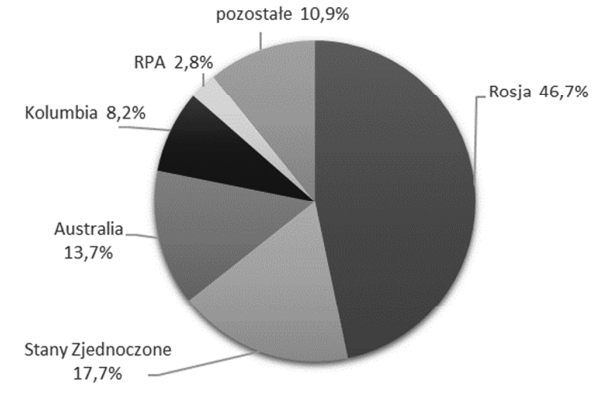
\includegraphics[width=0.6\textwidth]{./out_figures/figure_1}
  
    \captionsetup{margin=10pt,font=small,labelfont=bf,width=.8\textwidth}
    
  \caption[Źródła importu ropy naftowej do UE w 2019 roku (w \%)]{Źródła importu ropy naftowej do UE w 2019 roku (w \%). Źródło: \cite{pangsykania2022}}
  \label{fig:x1}
\end{figure}

Jak zaprezentowano na wykresie~\ref{fig:x1}, Rosja była najistotniejszym dostawcą ropy naftowej do UE w 2019 roku. Stany Zjednoczone zaspokajały blisko 18\% unijnego importu ropy naftowej. Istotnym dostawcą była także Australia, odpowiadająca niemal za 14\% importu omawianego surowca do Unii Europejskiej.

\begin{figure}[hbt]
  \centering

  \begin{subfigure}[t]{0.45\textwidth}
    \hspace{-0.4cm}
    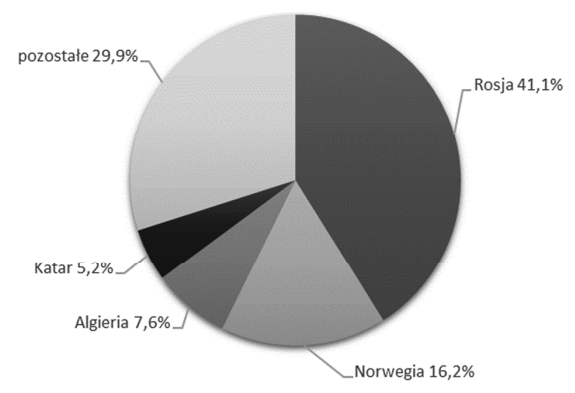
\includegraphics[width=1.12\textwidth]{./out_figures/figure_2}
  \end{subfigure}

  \captionsetup{margin=10pt,font=small,labelfont=bf,width=.8\textwidth}

  \caption[Źródła importu paliw stałych do UE w 2019 roku (w \%).]{Źródła importu paliw stałych do UE w 2019 roku (w \%). \textit{Źródło:} \cite{pangsykania2022}}\label{fig:x2}
\end{figure}

Jak wynika z wykresu~\ref{fig:x2}, największym dostawcą gazu ziemnego do UE w 2019 roku była Federacja Rosyjska. Znaczącymi dostawcami tego surowca były także: Norwegia, Algieria oraz Katar. 

Na wykresie~\ref{fig:x3} ukazano źródła importu paliw stałych do UE w 2019 roku. Najważniejszym źródłem importu paliw stałych do UE w tym roku była Federacja Rosyjska. Istotnymi dostawcami tych surowców były również: Irak, Nigeria, Arabia Saudyjska, Kazachstan, Norwegia, Libia, USA, Wielka Brytania, Azerbejdżan i Algieria. 

\begin{figure}[hbt]
  \centering

  \begin{subfigure}[t]{0.45\textwidth}
    \hspace{-1cm}
    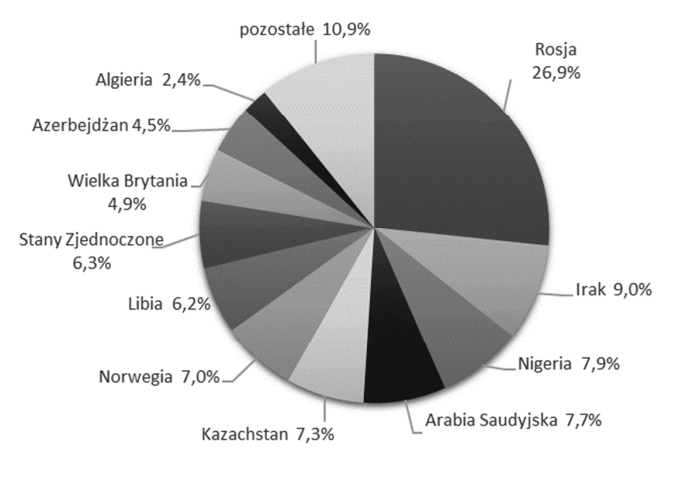
\includegraphics[width=1.3\textwidth]{./out_figures/figure_3}
  \end{subfigure}

  \captionsetup{margin=10pt,font=small,labelfont=bf,width=.8\textwidth}

  \caption[Źródła importu gazu ziemnego do UE w 2019 roku (w \%).]{Źródła importu gazu ziemnego do UE w 2019 roku (w \%). \textit{Źródło:} \cite{pangsykania2022}}\label{fig:x3}
\end{figure}

Ukazano także zależność energetyczną w krajach UE w 2019 roku (wykres~\ref{fig:x3}). Indykator zależności energetycznej pokazuje, w jakim stopniu dany kraj jest zależny od importu energii. Im niższy wskaźnik zależności energetycznej, tym niższy udział importowanych źródeł energii w całkowitym jej zużyciu. Jak wynika z danych zawartych na wykresie~\ref{fig:x3}, najbardziej niezależnym energetycznie krajem UE jest Estonia, dlatego że jej zależność energetyczna od importu surowców energetycznych wynosi --- według stanu na 2019 rok --- niespełna 5\%. Dla Polski indykator zależności energetycznej wynosi --- dla analizowanego, zunifikowanego okresu porównawczego --- 47\%. Dla porównania, skala zależności niemieckiej gospodarki od importu energii jest zdecydowanie wyższa i --- według stanu na 2019 rok --- wyniosła 67\% \citep{pangsykania2022}.

\begin{figure}[hbt]
  \centering

  \begin{subfigure}[t]{0.45\textwidth}
    \hspace{-1.8cm}
    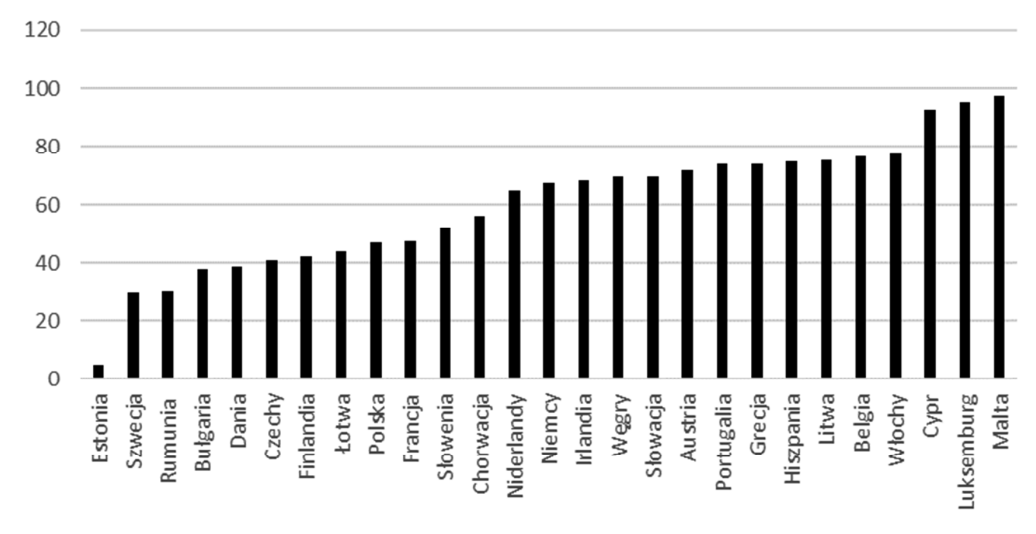
\includegraphics[width=1.4\textwidth]{./out_figures/figure_4}
  \end{subfigure}

  \captionsetup{margin=10pt,font=small,labelfont=bf,width=.8\textwidth}

  \caption[Indykator zależności energetycznej w krajach UE w 2019 (w \%).]{Indykator zależności energetycznej w krajach UE w 2019 (w \%). \textit{Źródło:} \cite{pangsykania2022}}\label{fig:x4}
\end{figure}

W okresie poprzedzającym wojnę ukraińsko-rosyjską polityka unijna ulegała zmianom w kierunku nadawania coraz większego znaczenia energii odnawialnej oraz zwiększania ekologiczności rozwiązań stosowanych w sektorze energetycznym. Jednocześnie, rozważano efektywność energetyczną, w obszarze której dążono do poprawy wydajności energetycznej, w tym poprzez oszczędność energii, jak i szeroką implementację rozwiązań energooszczędnych, a także obowiązkowe świadectwa energetyczne dla budynków, minimalne normy efektywności energetycznej dla różnych produktów, etykiety efektywności energetycznej i „inteligentne” liczniki. Po wybuchu wojny ukraińsko-rosyjskiej cele te zostały utrzymane, aczkolwiek istotnym kierunkiem stało się zwłaszcza uniezależnienie UE od surowców energetycznych z Federacji Rosyjskiej.

Ukazanie zasobów energetycznych UE, jak również skali zależności od importu surowców, pozwala przejść do struktury i regulacji rynku energii elektrycznej w UE. 


\subsubsection{Struktura i regulacje rynku energii elektrycznej w UE}

Najważniejszym dokumentem prawnym UE regulującym wspólnotowy rynek energii elektrycznej jest Rozporządzenie Komisji (UE) 2015/1222 z dnia 24 lipca 2015 roku \citep{ec2015} ustanawiające wytyczne dotyczące alokacji zdolności przesyłowych i zarządzania ograniczeniami przesyłowymi, przy czym dokument ten został zaktualizowany 15 marca 2021 roku i obowiązuje w wersji skonsolidowanej, po zmianach. 

Proces integracji rynku energii elektrycznej w UE zachodzi --- w myśl obowiązujących rozwiązań prawnych – dwutorowo, z jednej strony za pomocą oddolnych przedsięwzięć państw członkowskich w ramach kooperacji regionalnej oraz wspierania doskonalenia połączeń transgranicznych, z drugiej dzięki formowaniu unijnych ram prawnych, które nakładają na kraje członkowskie zobowiązanie implementowania konkretnych rozwiązań tak prawnych, jak i technicznych, przyczyniających się do efektywnej integracji z rynkiem unijnym. 

Unijny rynek energii elektrycznej złożony jest z następujących segmentów: rynku terminowego (Forward Market), Rynku Dnia Następnego (Day Ahead Market, RDN), Rynku Dnia Bieżącego (Intraday Market, RDB) oraz Transgranicznego rynku bilansującego (Cross-Border Balancing Market). Podstawowym rynkiem dla energii elektrycznej jest RDN. Funkcjonuje on na zasadzie: „dziś transakcja, jutro dostawa”, ponieważ zawierane na tym rynku transakcje powodują dostawę energii elektrycznej już w dniu następnym, po cenie wynegocjowanej w dniu transakcji. Istotność RDN polega także na tym, iż stanowi on punkt odniesienia dla cen energii elektrycznej w dowolnych innych kontraktach realizowanych na hurtowym rynku energii elektrycznej.

Rozporządzenie Komisji (UE) nr 2015/1222 z 24 lipca 2015 r., nazywane „rozporządzeniem CACM” \citep{ec2015} przyczyniło się do wdrożenia Nominowanego Operatora Rynku Energii Elektrycznej (NEMO). W myśl tego rozwiązania, w we wszystkich państwach członkowskich do 14 grudnia 2015 r. musiał zostać wyznaczony co najmniej jeden NEMO do realizacji jednolitej, spójnej synchronizacji rynków dnia następnego i bieżącego dla terenu rynkowego kraju. W Polsce status NEMO otrzymała Towarowa Giełda Energii. Najważniejszym zadaniem NEMO jest zapewnienie efektywnego działania fizycznego rynku spot energii elektrycznej w skali unijnej. NEMO przyjmuje i wykonuje oferty sprzedaży oraz kupna energii elektrycznej występujące na rynkach dnia następnego i bieżącego w obrocie międzynarodowym, wykonywane w ramach koncepcji synchronizowania rynków. 

W związku z dalekosiężnymi konsekwencjami pandemii, jak również kryzysem wywołanym wojną ukraińsko-rosyjską, UE adaptuje rozwiązania na rynku energii elektrycznej po to, aby zapewnić bezpieczeństwo tego rynku w całym obszarze unijnym. Najnowsze wyzwania UE w tym zakresie obejmują: redukcję zależności rachunków za energię elektryczną od krótkoterminowych cen paliw kopalnych, wspieranie rozwoju odnawialnych źródeł energii, usprawnienie funkcjonowania rynku w celu zapewnienia bezpieczeństwa dostaw oraz pełne wykorzystanie alternatyw dla gazu, takich jak magazynowanie i reakcja strony popytowej, zwiększenie ochrony i silnej pozycji konsumenta oraz udoskonalenie przejrzystości i integralności rynku oraz nadzoru nad nim sprawowanego \citep{ec2023}. 


\subsubsection{Analiza kluczowych wskaźników i trendów na rynku energetycznym w UE}

W 2021 roku wyznaczono cele w zakresie wydajności energetycznej do 2030 r. do 39\% w zakresie zużycia energii pierwotnej i 36\% w obszarze zużycia energii końcowej wobec prognoz z 2007 roku. Z powodu okoliczności stworzonych przez wojnę ukraińsko-rosyjską, w 2022 roku zmodyfikowano cele w ramach wydajności energetycznej, aby dostosować politykę energetyczną do wycofania importu rosyjskich paliw kopalnych. W efekcie, zdecydowano się na redukcję zużycia energii o minimum 13\% do 2030 r. --- wartości mierzonej wobec prognoz bazowych z 2007 r. (czyli w wartościach bezwzględnych do 750 mln ton ekwiwalentu ropy naftowej – Mtoe) i 980 Mtoe zużycia energii końcowej i pierwotnej w UE do 2030 r. Następnie rozpoczęto debatę nad lepszym dostosowaniem progów --- wysunięto m.in. koncepcję redukcji zużycia energii pierwotnej i końcowej w UE na poziomie 40–42\% i 36–40\% \citep{ep2023}.

Nieodłącznym elementem polityki energetycznej UE pozostaje zwiększanie znaczenia surowców odnawialnych w systemie energetycznym. Wzrost roli energii odnawialnej w platformie energetycznej wspólnoty wynika w dużej mierze z aspektów ekologicznych, ale nie tylko. Występowały prognozy, w świetle których na świecie występuje ograniczoność zasobów energetycznych nieodnawialnych --- i mimo że nawet te zasoby po pewnym czasie są w stanie w sprzyjających warunkach się odtwarzać --- to tempo ich zużywania przez współczesną cywilizację jest zbyt szybkie, a więc w konsekwencji, po pewnym czasie energetyczne zasoby nieodnawialne uległyby wyczerpaniu. Prawdopodobnie jednak największe znaczenie nadane rozwojowi polityki zwiększającej znaczenie surowców odnawialnych wynika z tego, że surowce odnawialne są ekologiczne, a zużywanie zasobów nieodnawialnych powoduje trwałe zmiany klimatu, jednoznacznie szkodliwe dla człowieka i ekosystemów życia na planecie dla roślin i zwierząt. Jest tak, szczególnie że w najbliższym czasie skończoność surowców nieodnawialnych nie stanowiła zagrożenia bezpośredniego dla cywilizacji, a więc najważniejszy argument na rzecz surowców odnawialnych zawarł się w ich ekologiczności \citep{ep2023}. 

W odpowiedzi na zagrożenia ekologiczne i klimatyczne, UE stara się więc rozwijać energię słoneczną, wiatrową, wodną oraz inne rozwiązania z zakresu energii odnawialnej. W znacznym stopniu rozwój ten wiąże się co prawda z dywersyfikacją źródeł energii, aczkolwiek w kierunku nie tylko zmian źródeł dostaw, co modyfikacji wewnętrznej sektora energetycznego, w którym --- niezależnie czy produkowana, czy też importowana energia --- będzie polegała w coraz większym zakresie na surowcach odnawialnych. W 2018 roku zaplanowano, iż odnawialne źródła energii będą do 2030 roku stanowiły minimum 32\% zasobów odpowiadających za produkcję energii w UE. Zgodnie ze stanowiskiem UE, zwiększana będzie rola m.in. energii morskiej z surowców odnawialnych. 

W maju 2022 roku wysunięto koncepcję aktualizacyjną, w świetle której wysunięty został pomysł, iż do 2030 roku energia ze źródeł odnawialnych wynosi do 45\% w całym unijnym systemie energetycznym. Założono m.in. podwojenie mocy fotowoltaicznych do 2025 r. Szczególnie istotne było jednak, iż zainicjowano wtedy trwałe wycofanie rosyjskich paliw kopalnych z rynku unijnego, co stanowiło reakcję na wojnę ukraińsko-rosyjską i brak wiarygodności Federacji Rosyjskiej na arenie międzynarodowej, w tym w zakresie sektora energetycznego. Komisja rozpoczęła wówczas współpracę z partnerami międzynarodowymi w celu dywersyfikacji dostaw i zabezpieczenia importu skroplonego gazu ziemnego (LNG) i większych dostaw gazu z rurociągów od partnerów międzynarodowych. Powstała wspólnotowa platforma energetyczna, będąca dobrowolnym mechanizmem koordynacji wspierającym zakup gazu i wodoru dla UE. Wysunięto wówczas także zewnętrzną strategię energetyczną UE uwzględniającą wsparcie Ukrainy, Mołdawii, Bałkanów Zachodnich i krajów Partnerstwa Wschodniego, jak również najsłabszych partnerów UE.

W maju 2022 roku pojawił się plan, który pozwolił zakończyć zależność UE od rosyjskich paliw kopalnych dzięki oszczędności energii, dywersyfikacji dostaw energii i przyspieszeniu wprowadzania energii ze źródeł odnawialnych. W czerwcu tego samego roku zaimplementowano rozwiązania w zakresie magazynowania gazu wprowadzające obowiązki w ramach minimalnych poziomów magazynowania tego surowca. W lipcu tego samego roku wdrożono skoordynowane środki redukcji popytu na gaz, zakładające ograniczenie zużycia gazu w Europie o 15\% w stosunku do poziomu z wiosny 2023 r. Wyznaczone zostały także zasady oszczędności na czas przejścia UE z surowców rosyjskich na zasoby z innych źródeł \citep{ep2023}. 

Jak widać, powody zmian w polityce energetycznej UE wiążą się ściśle z determinantami rozwoju sektora energetycznego wspólnoty. Uwarunkowania i kierunki zmian w dużej mierze zostały wyznaczone przez konflikt ukraińsko-rosyjski, ale nie tylko. Wojna ukraińsko-rosyjska spowodowała konieczność rezygnacji przez UE z rosyjskich paliw kopalnych oraz zakończenia współpracy z Rosją w sektorze energetycznym. Mimo poważnego wyzwania dla unijnego sektora energetycznego, którym stało się uniezależnienie od zasobów rosyjskich, UE była --- i jest --- w stanie także prowadzić efektywną politykę energetyczną w innych obszarach, w tym uwzględniających cele strategiczne nakreślone wcześniej, takie jak walka z kryzysem klimatycznym, dywersyfikacja źródeł energii oraz rozwijanie przedsięwzięć kluczowych w ramach infrastruktury energetycznej \citep{ep2023}. 



\subsection{Wpływ pandemii COVID-19 na rynek energetyczny w krajach Unii Europejskiej}
\subsubsection{Skutki lockdownów i ograniczeń na rynek energii elektrycznej}

Dnia 17 listopada 2019 roku w chińskim mieście Wuhan wybuchła epidemia wirusa SARS-CoV-2, która stała się następnie epidemią globalną COVID-19. Ostatniego dnia grudnia 2019 roku komisja ds. zdrowia w Wuhan poinformowała o nowym wirusowym zapaleniu płuc powodowanym przez nowo odkrytego wirusa. Dnia 11  marca  2020  roku  została  ogłoszona przez Światową Organizację Zdrowia (WHO) pandemia, czego powodem były: szybkie rozprzestrzenianie się wirusa na całym świecie, liczne zachorowania i ich przyrost w szybkim tempie oraz wysokie ryzyko zgonów osób zakażonych \citep{gorska2023}.

Tempo rozprzestrzeniania się COVID-19 było błyskawiczne --- jeszcze na początku marca 2020 roku odnotowano blisko 90 tysięcy zachorowań, zwłaszcza w Chinach, podczas gdy już po trzech tygodniach według danych WHO było 415 tysięcy zarażonych w 169 krajach na świecie oraz blisko 19 tysięcy zgonów z powodu wirusa odpowiadającego za epidemię. Polski rząd wprowadził stan zagrożenia epidemicznego 13 marca 2020 roku, a stan epidemii --- tydzień później, co wiązało się z implementowaniem restrykcji mających przeciwdziałać transmisji wirusa \citep{wajer2023}. 

Sektor elektroenergetyczny był tym, w którym wpływ COVID-19 wydawał się początkowo znikomy. W stosunku do marca 2019 roku, w marcu 2020 roku europejskie ceny energii elektrycznej spadły o €15/MWh, a ceny węgla --- o ponad \$20/tonę. Spadło także zużycie energii --- zarówno w Polsce, jak i innych krajach unijnych, jak Włochy, Hiszpania czy Niemcy. Spodziewano się już w marcu 2020 roku, że gwałtowny spadek aktywności gospodarczej modyfikujący światowy łańcuch dostaw, zredukowane wydatki na turystykę oraz podróże biznesowe, występujący okresowo deficyt zapasów, ograniczenie produkcji, zmniejszony popyt na największych rynkach oraz spodziewane lockdowny będą determinować konsekwencje de facto we wszystkich dziedzinach, obszarach i gałęziach gospodarki, także w sektorze elektroenergetycznym. Spodziewano się m.in., że --- mimo tymczasowego spadku cen energii – docelowo koszty jej pozyskania wzrosną, dlatego że nastąpi wyższa zmienność cen, motywowana niepewnością panującą na rynku. Prognozowano, że sektor elektroenergetyczny wykaże symptomy kryzysu w drugiej fali, ze względu na wpływ COVID-19 na klientów lub dostawców sektora elektroenergetycznego \citep{wajer2023}. 

Jeszcze w tym samym miesiącu pojawiły się głosy, iż pandemia koronawirusa wpływa na pracę zakładów przemysłowych, a w Europie spada zapotrzebowanie na energię. Spodziewane były już chwilowe przerwy w dostawach komponentów z Chin --- np. do farm słonecznych, wiatrowych i samochodów elektrycznych. Poza wdrażaniem zamknięcia lub prognozowaniem zamknięcia szkół, restauracji czy kin, zamykane były także --- lub prognozowano zamknięcie --- zakładów pracy, w tym fabryk. Największy koncern motoryzacyjny Volkswagen zamknął czasowo fabryki w Europie, podobnie stało się w Hiszpanii z Renault, a we Francji i Hiszpanii zawiesił produkcję lotniczy Airbus. W takich okolicznościach, zapotrzebowanie na energię malało \citep{wysokienapiecie2023}. 

W czerwcu 2020 roku ograniczenia w funkcjonowaniu gospodarki, zostały wprowadzone w celu powstrzymania rozwoju pandemii, przyczyniły się do utrzymania procesu spadku zapotrzebowania na energię elektryczną. W Polsce, w początkowym okresie obostrzeń spadek ten wyniósł blisko 10\%, aczkolwiek już w czerwcu 2020 roku malał. W wielu krajach unijnych skala zmian była większa --- we Włoszech w początkowym stadium pandemii odnotowano dwukrotnie niższe zapotrzebowanie na energię elektryczną. W Polsce, wraz ze spadkiem zapotrzebowania na energię, jej ceny zmalały. Wobec klientów prosumenckich spadek popytu na energię z sieci zaczął przyczyniać się do nowych kosztów po stronie systemu energetycznego. Malejąca liczba odbiorców, którzy ponosili opłaty dystrybucyjne oznaczała, że należało je dzielić na mniejszą liczbę podmiotów, a w efekcie --- rosła jednostkowa wzrasta. Pojawiły się także nowe problemy techniczne, związane z pracą sieci. Pojawiło się wyzwanie w postaci konieczności magazynowanie energii \citep{ure2023}.

Mimo początkowych spadków cen energii i zapotrzebowania na nią, powodowanych przez pandemię oraz obostrzenia wprowadzone przeciwko niej, w dłuższym horyzoncie czasu pojawiły się problemy z niestabilnymi cenami energii. W szczególności, wzrosło ubóstwo  energetyczne, rozumiane jako „sytuacja, w której gospodarstwo domowe lub osoba nie ma możliwości uzyskania podstawowych usług energetycznych (oświetlenie, ogrzewanie, chłodzenie, mobilność i energia elektryczna) zapewniających godny poziom życia, ze względu na połączenie niskiego dochodu, wysokich wydatków na energię i niskiej efektywności energetycznej  mieszkań” \citep{gorska2023}. Problemem upowszechnionym stało się deficyt zasobów na utrzymanie ogrzewania na odpowiednim poziomie za uczciwą cenę \citep{gorska2023}. 


\subsubsection{Analiza zmian w zużyciu prądu w okresie pandemii}

Średnie zapotrzebowanie na prąd w Polsce w szesnastym tygodniu 2020 roku zmniejszyło się w porównaniu do analogicznego okresu roku ubiegłego o 12,38\% (wykres~\ref{fig:x5}). W piętnastym tygodniu spadek wynosił 15,54\%. Do drugiej połowy kwietnia 2020 roku średnie zapotrzebowanie na prąd w Polsce było o 4,52\% niższe niż w analogicznym okresie 2019 roku. Po piętnastu tygodniach spadek wynosił 4,04\% \citep{biuroanalizpfr2020}.

\begin{figure}[hbt]
  \centering

  \begin{subfigure}[t]{0.45\textwidth}
    \hspace{-1.8cm}
    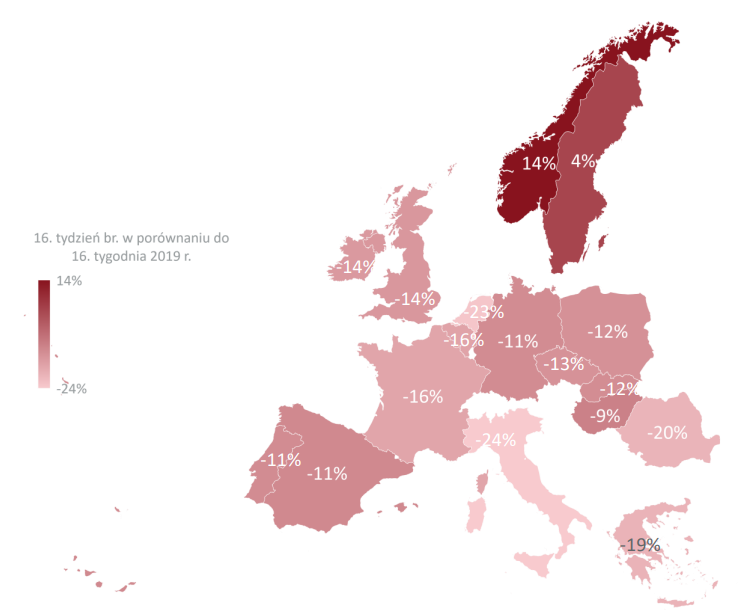
\includegraphics[width=1.4\textwidth]{./out_figures/figure_5}
  \end{subfigure}

  \captionsetup{margin=10pt,font=small,labelfont=bf,width=.8\textwidth}

  \caption[Zmiany zapotrzebowania na energię elektryczną (1 tydzień)]{ Zestawienie szesnastego tygodnia 2020 r. do analogicznego okresu 2019 r. w zakresie zmian zapotrzebowania na energię elektryczną. \textit{Źródło:} \cite{biuroanalizpfr2020}}\label{fig:x5}
\end{figure}

Największy spadek zapotrzebowania na energię elektryczną do drugiej połowy kwietnia 2020 roku odnotowano --- w porównaniu do 2019 roku --- we Włoszech (-11\%). Z drugiej strony, zarejestrowany został wzrost w Irlandii (+1\%). Dane te ukazano na wykresie~\ref{fig:x6}. 

\begin{figure}[hbt]
  \centering

  \begin{subfigure}[t]{0.45\textwidth}
    \hspace{-1.8cm}
    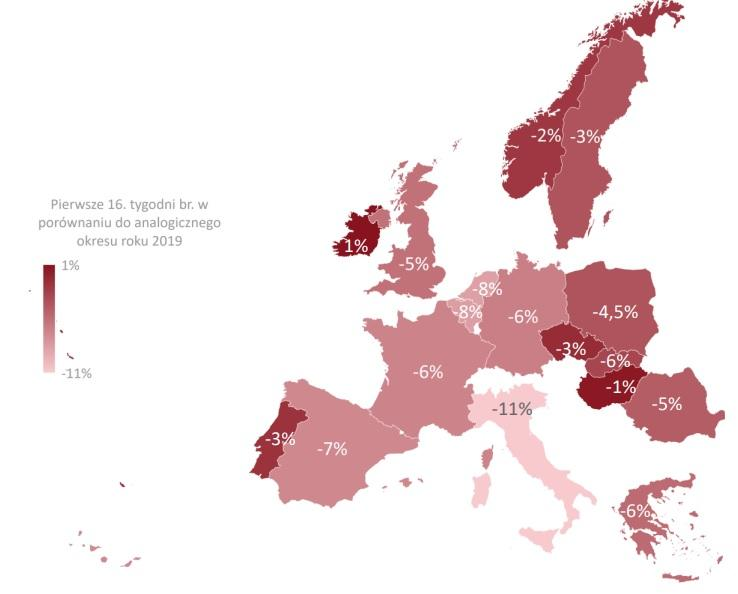
\includegraphics[width=1.4\textwidth]{./out_figures/figure_6}
  \end{subfigure}

  \captionsetup{margin=10pt,font=small,labelfont=bf,width=.8\textwidth}

  \caption[Zmiany zapotrzebowania na energię elektryczną (16 tygodni)]{Zestawienie pierwszych szesnastu tygodni 2020 r. do analogicznego okresu 2019 r. w zakresie zmian zapotrzebowania na energię elektryczną. \textit{Źródło:} \cite{biuroanalizpfr2020}}\label{fig:x6}
\end{figure}

W czasie lockdownu w 2020 r., z powodu restrykcji ograniczających działalność gospodarczą, nastąpiła redukcja poboru energii elektrycznej na poziomie krajowego systemu elektroenergetycznego. Jakkolwiek, odmienną specyfiką wyróżniła się grupa odbiorców mieszkaniowych --- w ich zakresie trendem stał się, z powodu pandemii, wzrost zużycia energii w porównaniu z okresem sprzed niej \citep{artsmart2023}. 

Konieczność relokacji aktywności zawodowych, towarzyskich oraz społecznych, a także edukacji do domów w czasie pandemii spowodowała modyfikacje w profilu użytkowania energii elektrycznej. W badaniu na informacjach pozyskanych z 7000 liczników inteligentnych zainstalowanych u odbiorców mieszkaniowych na obszarze warszawskich osiedli w budynkach wielorodzinnych powstałych po 2005 r., przy czym zarazem --- danych pozyskanych od 16 marca do 18 kwietnia 2020 r. (w okresie narodowej kwarantanny) oraz od 16 marca do 18 kwietnia 2018 r. (w okresie analogicznym sprzed pandemii) okazało się, że zapotrzebowanie na energię w pandemii wzrosło, zwłaszcza w godzinach od 9.00 do 19.00, a w pozostałych godzinach generalnie utrzymywało się na podobnym poziomie, jak w okresie przed pandemią. Jednocześnie, występował stabilny poziom uśrednionej mocy szczytowej w 1-godzinnym interwale przeciętnego odbiorcy energii elektrycznej, niezależnie od tego, czy odbiorca przebywał w domu, czy też nie \citep{artsmart2023}. 

Uwzględniając i generalizując dane z całego kraju, należy powiedzieć, iż lockdown w pierwszej fazie pandemii zdecydowanie zmniejszył krajowe zużycie energii elektrycznej, ale już w swojej listopadowej odsłonie zaczął zwiększać zapotrzebowanie --- przynajmniej użytkowników domowych --- na energię elektryczną \citep{kazimierska2023}.

Przyrost zapotrzebowania na energię elektryczną wśród użytkowników domowych nie zrekompensował jednak spadku zapotrzebowania na energię elektryczną wśród innych użytkowników, w tym przedsiębiorstw produkcyjnych i handlowych --- i tak było w całej Unii Europejskiej. W 2022 roku co prawda, mimo kryzysu energetycznego, popyt na energię elektryczną wzrósł na całym świecie blisko o 2\%. Jednak w Europie w tym czasie odnotowano zdecydowany spadek zapotrzebowania na energię elektryczną --- aż o 3\%. W Europie był to bardzo wysoki spadek roczny zapotrzebowania na tę energię. Większy spadek zdarzył się tylko w czasie pandemii, w okresie 2020--2021 --- uwzględniając dane od czasu kryzysu finansowego z lat 2008-2009 \citep{maciuch2023}.  

\subsubsection{Porównanie danych przed pandemicznych i okresu pandemii}

Jak wynika z analizy danych obciążenia Krajowego Systemu Elektroenergetycznego zgromadzonych przez Polskie Sieci Elektroenergetyczne, uwzględniających wartości popytu na moc i jego prognozę w poszczególnych godzinach w odniesieniu do wartości tygodniowych dla dni roboczych i tygodni 11--22 okresu 2017--2019 i roku pandemicznego 2020 (przy czym tygodnie 11--13 przypadają na marzec, 14--18 na kwiecień, a 19--22 --- na maj), w latach 2017--2019 zauważyć można naturalne, sukcesywne obniżanie się wartości szczytowych, będącego rezultatem sezonowych zmian zapotrzebowania na moc, natomiast w 2020 roku, w tygodniach 11--14 nastąpił znaczący spadek tych wartości, co wiązało się z rosnącym przyrostem zachorowań oraz implementowaniem ograniczeń w funkcjonowaniu gospodarki i społeczeństwa \citep{stahl2021}. 

Szczytowe obciążenie w marcu 2020 roku uległo redukcji średnio o ok. 1000 MW (4\%). W następnych tygodniach wartości szczytów tygodniowych były mniejsze średnio o ok. 2000 MW (9\%) względem poprzednich lat. Mimo stopniowego znoszenia restrykcji od tygodnia 19, obciążenia szczytowe nie zbliżyły się do obciążeń dla okresu porównawczego --- były niższe o ok. 1200 MW (6\%). W rezultacie wprowadzonych restrykcji zamykano zakłady pracy, ograniczano ich działalność, wprowadzano przerwy i przestoje, liczne firmy zredukowały produkcję, co w następstwie powodowało zmiany zapotrzebowania na energię elektryczną. Z powodu ograniczeń z zakresu produkcji i konsumpcji, w drugim kwartale 2020 roku polska gospodarka straciła 8\% PKB. Prawdopodobnie, występujące problemy spowodowały zredukowane zapotrzebowanie na moc w kolejnych tygodniach w porównaniu z poprzednimi latami \citep{stahl2021}. 

\begin{figure}[hbt]
  \centering

  \begin{subfigure}[t]{0.45\textwidth}
    \hspace{-1.5cm}
    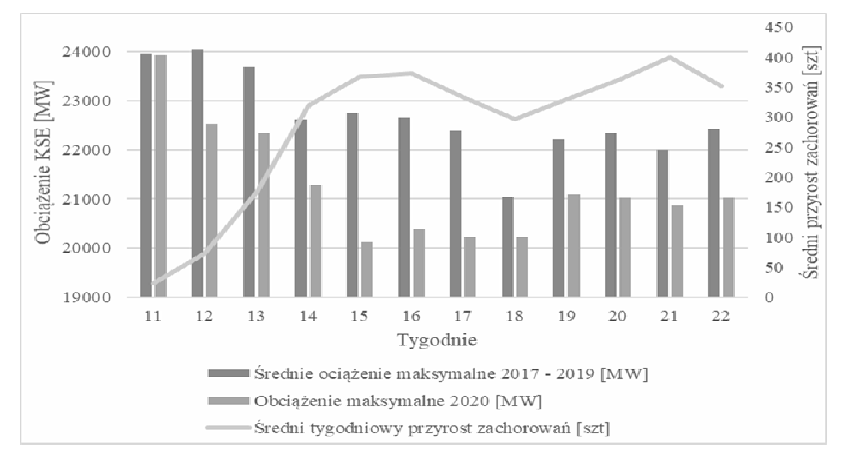
\includegraphics[width=1.4\textwidth]{./out_figures/figure_7}
  \end{subfigure}

  \captionsetup{margin=10pt,font=small,labelfont=bf,width=.8\textwidth}

  \caption[Szczytowe zapotrzebowanie na moc w poszczególnych tygodniach w latach 2017--2019 oraz w roku pandemicznym 2020]{Szczytowe zapotrzebowanie na moc w poszczególnych tygodniach w latach 2017--2019 oraz w roku pandemicznym 2020 --- maksymalne obciążenie oraz średni przyrost zachorowań na COVID-19. \textit{Źródło:} \cite{stahl2021}}\label{fig:x7}
\end{figure}

Na wykresie~\ref{fig:x7} ukazano szczytowe zapotrzebowanie na moc w poszczególnych tygodniach w latach 2017--2019 oraz w roku pandemicznym 2020. Dane te, maksymalne obciążenie zostały odniesione do średniego przyrostu zachorowań na COVID-19. Natomiast na wykresie~\ref{fig:x8} zaprezentowano minimalne obciążenie w tygodniach 2017--2019 i roku pandemicznym 2020 oraz średni przyrost zachorowań na COVID-19. 

Jak wynika z zaprezentowanych danych, największa różnica między minimalnymi obciążeniami wystąpiła w tygodniu 16. W roku 2020 minimalne obciążenie było mniejsze niż w latach 2017--2019 średnio o ok. 500 MW (4\%).

\begin{figure}[hbt]
  \centering

  \begin{subfigure}[t]{0.45\textwidth}
    \hspace{-1.5cm}
    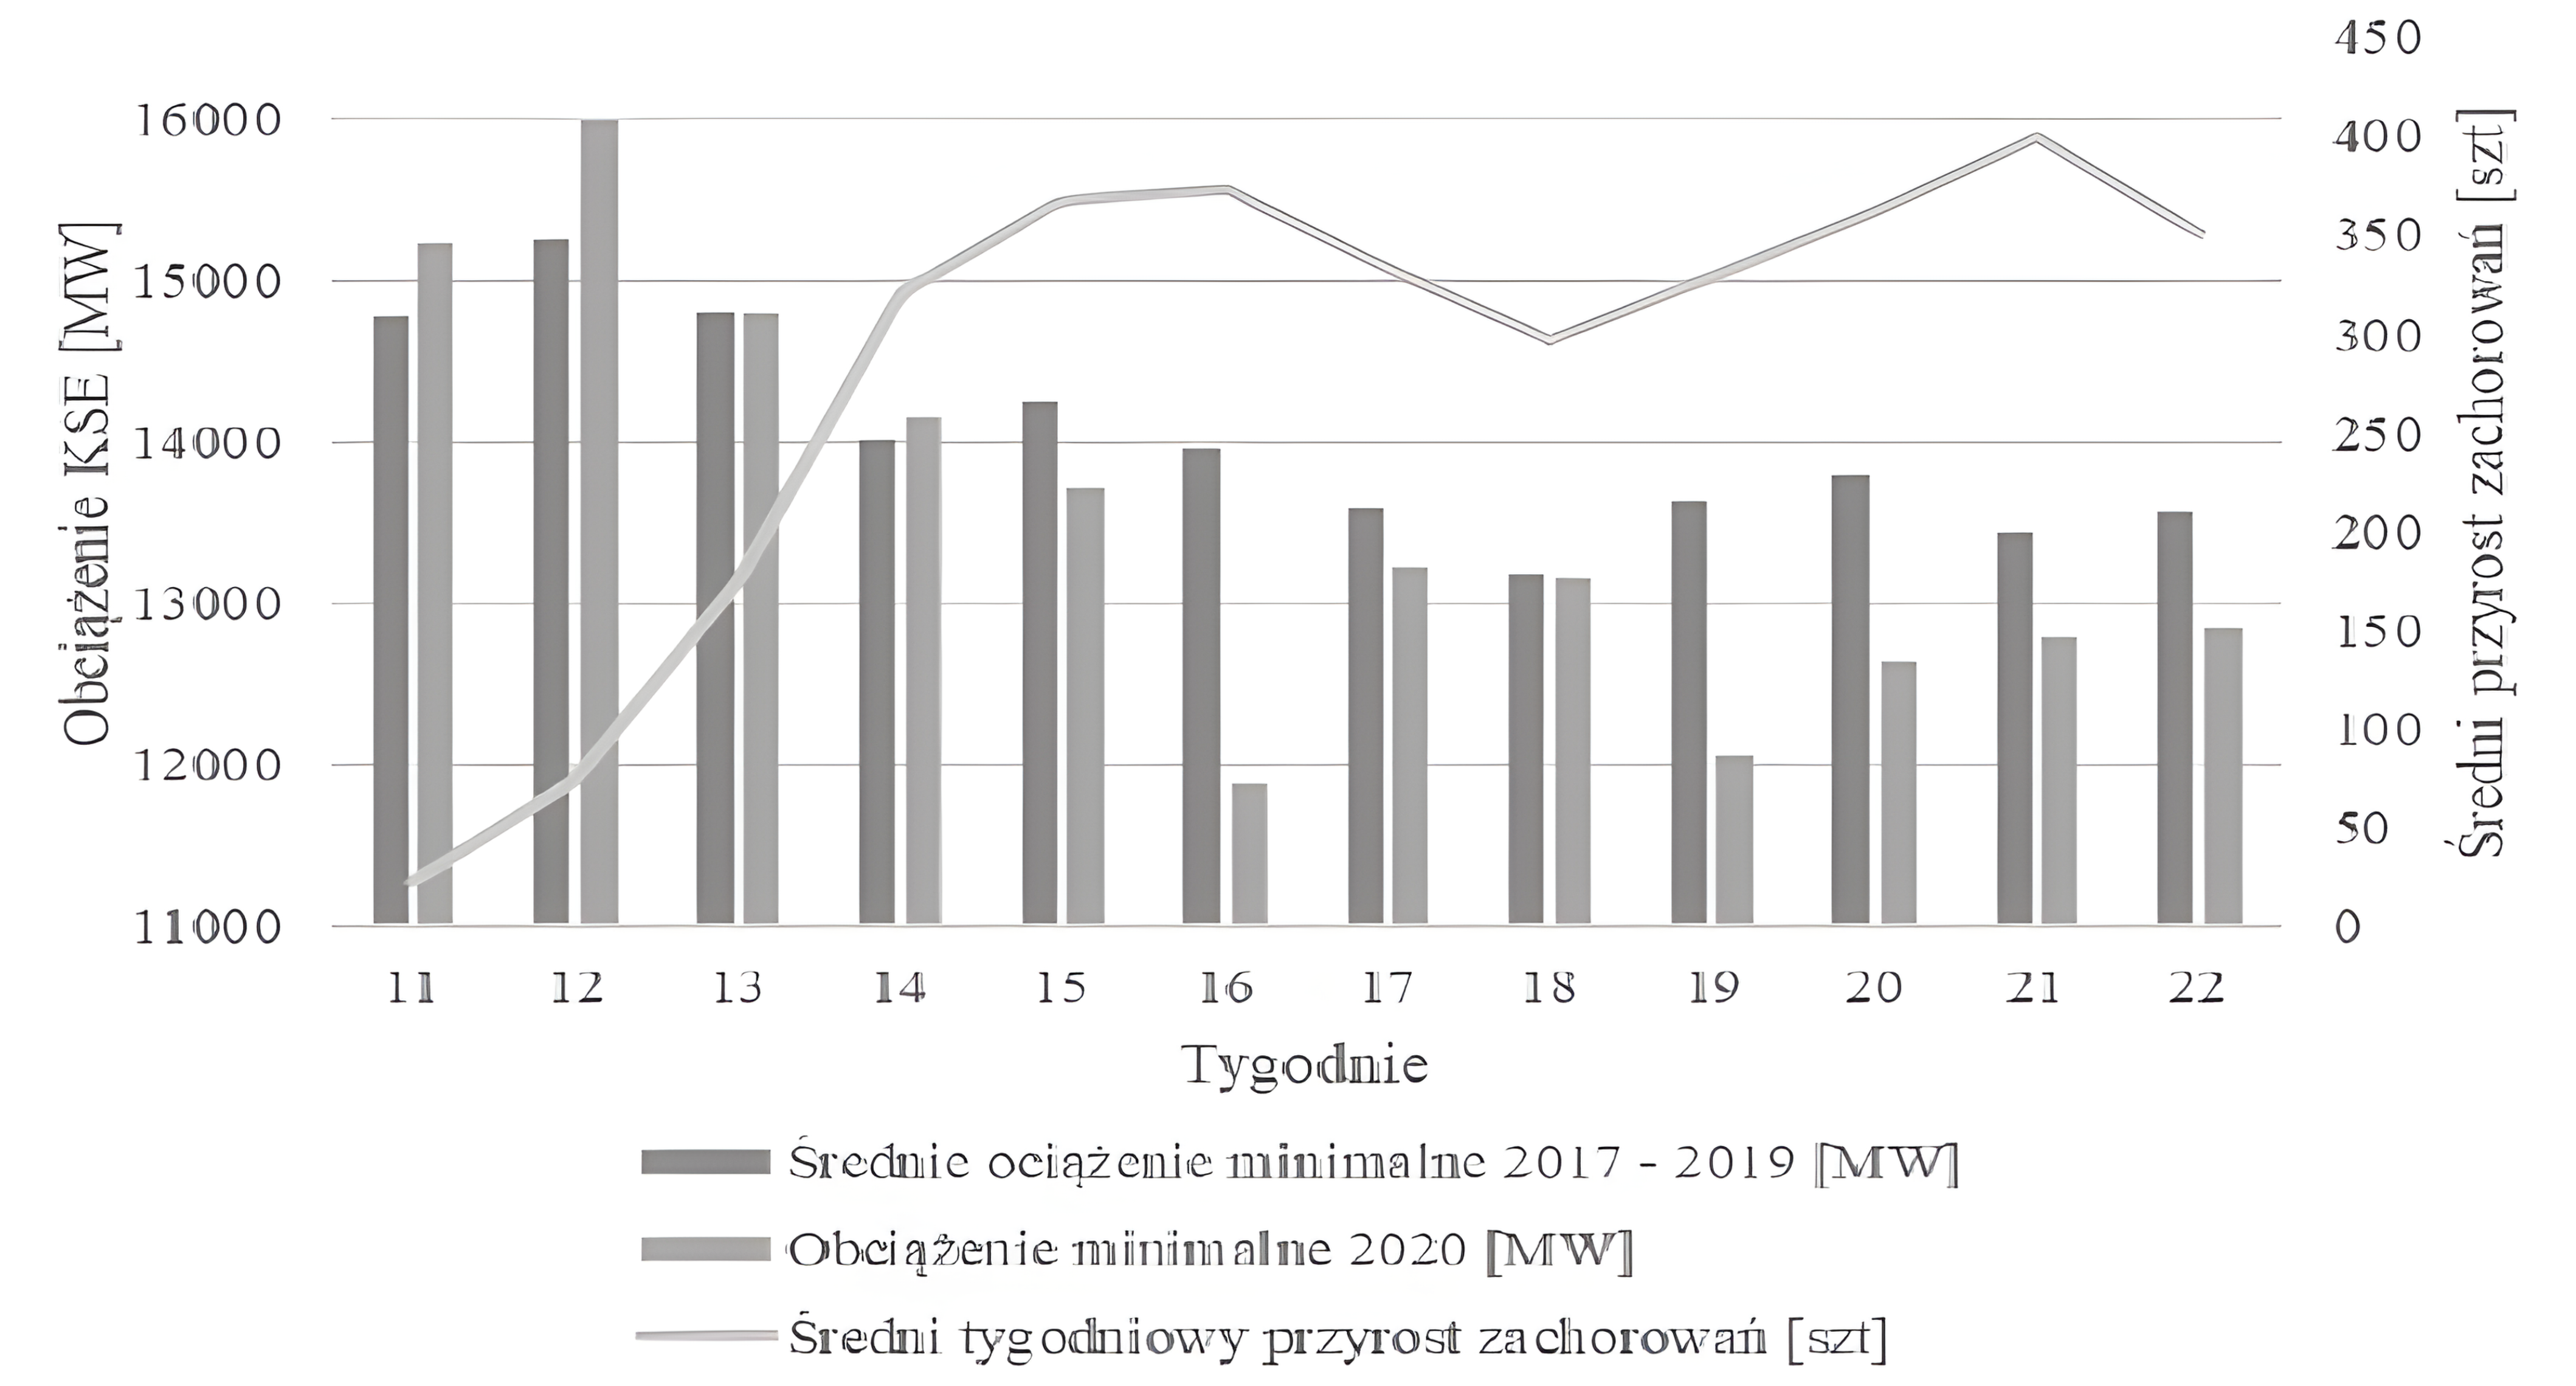
\includegraphics[width=1.4\textwidth]{./out_figures/figure_8}
  \end{subfigure}

  \captionsetup{margin=10pt,font=small,labelfont=bf,width=.8\textwidth}

  \caption[Minimalne obciążenie w tygodniach 2017--2019 i 2020 roku oraz średni przyrost zachorowań na COVID-19]{Minimalne obciążenie w tygodniach 2017--2019 i 2020 roku oraz średni przyrost zachorowań na COVID-19. \textit{Źródło:} \cite{stahl2021}}\label{fig:x8}
\end{figure}

Z przytoczonego badania wynika także, że średnie tygodniowe obciążenia w okresie lockdownu wykazały spadek zapotrzebowania o ok. 1300 MW (7\%). W wyniku restrykcji zredukowane zostały nie tylko obciążenia szczytowe, ale także ogólny popyt na moc \citep{stahl2021}.

Mimo spadku zapotrzebowania na energię elektryczną spowodowanego przez pandemię, pandemia przyczyniła się jednocześnie do wzrostu cen energii za prąd. Wzrost ten objawia się rosnącymi na całym globie, nie tylko w Unii Europejskiej, hurtowymi cenami energii. De facto wzrost ten został zapoczątkowany w 2021 roku, a więc w drugim roku pandemicznym --- w rezultacie dalekosiężnego, długofalowego i przedłużającego się negatywnego wpływu pandemii na gospodarkę i społeczeństwo. W 2022 roku rosyjska inwazja na Ukrainę oraz dynamicznie zmieniające się warunki klimatyczne zaostrzyły kryzys w sektorze energetycznym, wyłaniając kolejne czynniki wzrostu cen \citep{council2023}. 

Między grudniem 2020 r. a grudniem 2021 r. importowe ceny energii w strefie euro uległy dwukrotnemu zwiększeniu. Wzrost ten był spektakularny, zwłaszcza że importowe ceny energii, mimo ze podatne na fluktuacje, z zasady nie zmieniają się o więcej niż 3/10 w skali roku. Kryzys wywołany przez pandemię wzmocniony został przez wojnę ukraińsko-rosyjską, która wybuchła w lutym 2022 roku oraz przez falę upałów w lecie tego samego roku \citep{council2023}). Na wykresie 7 ukazano dane z całej UE od stycznia 2021 r. do stycznia 2023 r. w zakresie cen energii u producentów przemysłowych oraz konsumpcyjnych cen energii elektrycznej, gazu i innych paliw.


\begin{figure}[hbt]
  \centering

  \begin{subfigure}[t]{0.45\textwidth}
    \hspace{-1.5cm}
    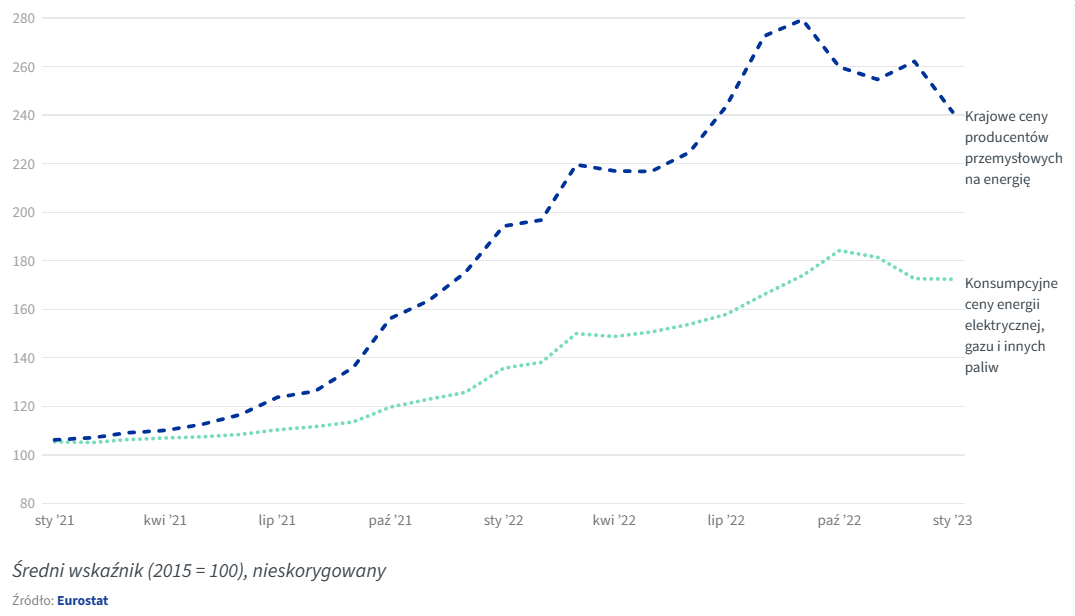
\includegraphics[width=1.4\textwidth]{./out_figures/figure_9}
  \end{subfigure}

  \captionsetup{margin=10pt,font=small,labelfont=bf,width=.8\textwidth}

  \caption[Producenckie i konsumpcyjne ceny energii w Unii Europejskiej w okresie 2021--2023]{Producenckie i konsumpcyjne ceny energii w Unii Europejskiej w okresie 2021--2023. \textit{Źródło:} \cite{council2023}}\label{fig:x9}
\end{figure}

Jak widać na wykresie~\ref{fig:x9}, ceny energii w całej UE rosną. W 2022 roku ceny te osiągnęły rekordowy poziom. W 2023 roku nastąpił co prawda pewien spadek cen energii na obszarze unijnym, co wynikało z polityki unijnej w sektorze energetycznym prowadzącej do dywersyfikacji źródeł surowców energetycznych, aczkolwiek nie jest pewne, na ile tendencja hamująca ceny energii jest stała. Wartość cen energii w UE jest w 2023 roku i tak znacząco wyższa niż w 2021 roku, gdy zaczęły uwidaczniać się najpoważniejsze następstwa pandemii dla sektora energetycznego. 
\subsection{Wpływ zmian w sektorze energetycznym spowodowanych przez pandemię COVID-19 na ekonomię w krajach UE}

\subsubsection{Skutki pandemii na gospodarkę krajów UE}

Na przełomie lat 2019--2020, a więc jeszcze przed ogłoszeniem pandemii, ale już w reakcji na pierwsze poważne doniesienia o spodziewanej ekspansji epidemii COVID-19, gospodarka światowa doznała spowolnienia. W miarę upływu czasu, ujemne skutki gospodarcze zaczęły, w większym lub mniejszym stopniu, obejmować dowolne kraje członkowskie Unii Europejskiej i świata.  

W styczniu i lutym 2020 roku nastąpiła redukcja aktywności gospodarczej Chin w rezultacie rozprzestrzeniającego się tam COVID-19, co wywarło wpływ także na inne kraje na świecie. Nastąpił de facto szok podażowy związany z dezorganizacją funkcjonujących wówczas łańcuchów dostaw, jak również szok popytowy skorelowany zarówno ze spadkiem popytu na dobra ze strony konsumentów, jak i --- z modyfikacjami planów inwestycyjnych przedsiębiorstw w związku z niepewnością dalszych uwarunkowań działania \citep{dziembala2021}. 

W miarę upływu czasu, wraz z rozprzestrzenianiem się najpierw epidemii, a następnie pandemii, nastąpiła redukcja płynności finansowej organizacji komercyjnych na całym świecie, nie tylko w UE. Pandemia spowodowała niewątpliwie pojawienie się kolejnych, rozmaitych szoków gospodarczych, w tym szoku medycznego, wynikającego z nieobecności w pracy osób chorych z powodu COVID-19. Szczególnie silny wpływ na gospodarkę miały czynności podejmowane przez rządy i inne podmioty decyzyjne w zakresie prób ograniczeń transmisji koronawirusa. Jakkolwiek, gdyby takie aktywności nie były podejmowane, pandemia mogłaby spowodować --- hipotetycznie --- nawet zagładę ludzkości. Gruntownym zmianom uległy postawy konsumentów oraz stanowiska przedsiębiorstw w ramach nastawienia do gospodarki --- w zależności od szczegółowych uwarunkowań przebiegu pandemii, zaczęły dominować koncepcje pesymistyczne lub zachodził zwrot w kierunku optymizmu. Aktywność zarówno przedsiębiorstw, jak i konsumentów na rynku uległy generalnie zmniejszeniu. 

Pandemia zaburzyła globalne łańcuchy dostaw. Wpłynęła silnie zwłaszcza na poszczególne branże, jak turystyka, gastronomia oraz usługi hotelowe, ale w związku z rozmiarem sytuacji pandemicznej, zagrożeniami przez pandemię niesionymi oraz obostrzeniami wprowadzonymi przeciwko rozprzestrzenianiu się konsekwencji pandemii, choćby pośrednio wywarła wpływ na wszystkie dziedziny życia tak ekonomicznego, jak i społeczno-kulturowego oraz gałęzie gospodarki. Pandemia przyczyniła się do utraty miejsc pracy oraz wzrostu ubóstwa. Skutki gospodarcze pandemii ujawniły się także przez wzgląd na konieczność ponoszenia przez władze państw (i władze administracji zdecentralizowanej) ogromnych wydatków na przeciwdziałanie transmisji koronawirusa. Spadające przychody firm komercyjnych korelowały w pandemii ze spadkiem ich dochodowości, co w rezultacie ograniczało możliwości inwestycyjne oraz ekspansję, jak również powodowało mniejsze wpływy podatkowe sektora publicznego \citep{dziembala2021}.  

W wyniku wprowadzonych lockdownów mających na celu powstrzymywanie transmisji wirusa, zdecydowanemu ograniczeniu uległa mobilność członków społeczeństwa. Negatywne skutki objęły kolejne branże, jak np. transportową. Mobilność członków społeczeństwa została zredukowana znacząco już w okresie od marca do maja 2020 roku, a więc na początku pandemii. Zamykane były fabryki i inne przedsiębiorstwa, następowały liczne, wydłużające się przestoje w pracy oraz produkcji, dochodziło do częstych nieobecności członków kadry pracowniczej. Panująca powszechnie niepewność i deficyty ekonomiczne przyczyniły się do spadku wydatków np. gospodarstw domowych. 

Niepożądane skutki pandemii dla gospodarki ujawniły się już w danych za pierwszy kwartał 2020 roku. Wtedy gospodarka unijna uległa po raz pierwszy spowolnieniu po czasie nieprzerwanego wzrostu trwającego od blisko siedmiu lat. Ograniczenie działalności gospodarczej i pozostałe skutki pandemii przyczyniły się do pogorszenia wyników ekonomicznych jeszcze bardziej w drugim kwartale 2020 roku. Wtedy nastąpiła redukcja PKB UE o 11,9\%, a w samej strefie euro --- o 12,1\% w zestawieniu do pierwszego kwartału tego samego roku, w którym i tak odnotowano spowolnienie wobec ostatniego kwartału 2019 roku (o 3,2\%), a więc w porównaniu do danych zniekształconych już przez pandemię. Oznaczało to definitywnie nasilanie się ujemnych skutków dla gospodarki unijnej. Największe spadki w drugim kwartale 2020 roku odnotowały: Hiszpania (-18,5\%), Portugalia (-14,1\%) i Francja (-13,8\%), ale wszystkie kraje unijne doznały konsekwencji gospodarczych z uwagi na sytuację pandemiczną \citep{dziembala2021}. 

Z powodu pandemii, w sposób niepożądany kształtowały się także indykatory rynku pracy. W czerwcu 2020 r. stopa bezrobocia wyniosła 7,8\% w strefie euro, a w całej UE --- 7,1\%. Niepożądanymi skutkami pandemii na rynku pracy objęci zostali zwłaszcza ludzie młodzi, wśród których stopa bezrobocia wyniosła 16,8\% w UE, a w strefie euro --- 17\% w lipcu 2020 roku \citep{dziembala2021}.

\subsubsection{Związki między zużyciem prądu a wskaźnikami ekonomicznymi}

Spadającym w pandemii wskaźnikom ekonomicznym towarzyszyły m.in. zmiany w zakresie zużycia prądu. Korelacja ta wynikała z tego, iż redukcja indykatorów ekonomicznych była powodowana przez ograniczenia wynikłe z pandemii i obostrzeń przeciwko rozprzestrzenianiu się koronawirusa, a w warunkach słabszych rezultatów gospodarczych osiąganych w takich okolicznościach, ujawniających się za pomocą spadających wskaźników ekonomicznych, firmy zużywały mniej prądu --- występowały przestoje, a nawet czasowe zamknięcia miejsc pracy i produkcji, co zmniejszało wielkość eksploatacji prądu. W 2020 roku zaobserwowana została zdecydowana redukcja wartości szczytowych zużycia prądu. O zmianach w popycie na prąd świadczyło także narastanie obciążenia w okresie szczytu popołudniowego. W 2020 roku pojawiające się zmiany w popycie na prąd stały się bardziej gwałtowne niż w okresie przed pandemią \citep{stahl2021}. 

W czerwcu 2020 roku zauważono, że wielkość zapotrzebowania na energię zależna będzie głównie od wdrożonych zaleceń zdrowotnych przeciwko koronawirusowi, czasu ich trwania oraz rygorystyczności. W zakresie wstępnych szacunków prognozowano spadek zużycia energii o około 6,0\% do końca 2020 roku, co odpowiadało łącznemu zużyciu Francji, Niemiec, Włoch oraz Wielkiej Brytanii. Tak więc, prognozowano już wtedy spadek siedmiokrotnie wyższy od spadku odnotowanego w okresie ogólnoświatowego kryzysu finansowego z 2008 roku. Tak znaczące obniżenie zapotrzebowania na energię nie miało precedensu w siedemdziesięciu latach poprzedzających wybuch pandemii \citep{kolenda2020}. 

Spadający popyt na energię w zakładach pracy był częściowo rekompensowany wzrostem zapotrzebowania na energię przez gospodarstwa domowe \citep{cire2023}. Wzrost zapotrzebowania na energię przez gospodarstwa domowe wynikał ze zwiększenia ilości czasu spędzanego w domach przez rodziny i inne komórki społeczne --- przede wszystkim był to efekt ograniczeń wprowadzonych w związku z zapobieganiem rozprzestrzenianiu się koronawirusa. Członkowie społeczeństwa więcej czasu spędzali w domach także dlatego, iż spopularyzowana została w warunkach pandemii praca w domu, za pomocą środków komunikacji na odległość --- telepraca. 

Ze względu na relatywnie nieduże modyfikacje ilościowej eksploatacji nośników energii w okresie 2002--2021 przez gospodarstwa domowe --- z wyjątkiem jednak energii elektrycznej właśnie (wzrost o 20,9\% w całym przytoczonym okresie), a poza tym także drewna opałowego (wzrost o 26\%), zwiększenie nakładów na nośniki energii wynikało ze znacznego wzrostu cen nośników energii. Zwiększenie średnich nominalnych wydatków gospodarstwa domowego w okresie 2002--2021 wyniosło 141,8\% dla węgla kamiennego i 143,3\% dla gazu ziemnego. Najpoważniejszym czynnikiem takich wzrostów była pandemia COVID-19, ponieważ ona zdeterminowała --- w skali długofalowej --- zwiększenie cen paliw i surowców tak na rynkach światowych, jak i unijnym oraz krajowym. W zakresie energii elektrycznej wzrost wydatków gospodarstw domowych w okresie 2002--2021 wyniósł 129,4\% i wynikał z dwóch wiodących przyczyn: zwiększenia zapotrzebowanie gospodarstw domowych na prąd oraz wzrostu cen tego nośnika energii. Natomiast zwiększenie wydatków na ciepło wyniosło w analizowanym okresie zaledwie 29,9\%, co wyniknęło z relatywnie niewielkiego wzrostu jego realnej ceny w tym czasie (a poza tym, ze zmniejszenia zużycia ciepła przez gospodarstwa domowe dzięki aktywnościom termomodernizacyjnym) \citep{gus2023}. 

\begin{figure}[hbt]
  \centering

  \begin{subfigure}[t]{0.45\textwidth}
    \hspace{-1.7cm}
    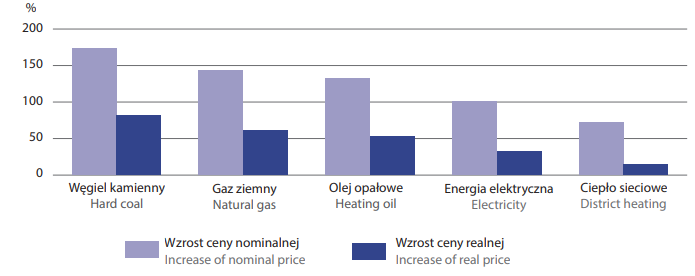
\includegraphics[width=1.43\textwidth]{./out_figures/figure_10}
  \end{subfigure}

  \captionsetup{margin=10pt,font=small,labelfont=bf,width=.8\textwidth}

  \caption[Wzrost cen nośników energii w ujęciu nominalnym i realnym w latach 2002--2021 w Polsce.]{Wzrost cen nośników energii w ujęciu nominalnym i realnym w latach 2002--2021 w Polsce. \textit{Źródło:} \cite{gus2023}}\label{fig:x10}
\end{figure}

Na wykresie~\ref{fig:x10} ukazano wzrost cen nośników energii w ujęciu nominalnym i realnym w latach 2002--2021 w Polsce. Wzrost ten został w dużej mierze spowodowany przez pandemię, którą ogłoszono w 2020 roku. Rosnące wydatki na nośniki energii stanowiły w 2021 roku znaczące obciążenie finansowe dla wszystkich grup społeczno-ekonomicznych gospodarstw domowych i miały kluczowe znaczenie w wydatkach na użytkowanie mieszkania i nośniki energii, co --- przy spadających wskaźnikach ekonomicznych w gospodarce --- było szczególnie niekorzystne. 

W zakresie wydatków gospodarstw domowych ogółem, istnieje możliwość spostrzeżenia od 2002 roku nieregularnego trendu wzrostowego udziału wydatków na energię. Największy wzrost odnotowano co prawda w 2011 roku --- wtedy wzrost wyniósł aż 12,2\%. Jednak w latach 2012--2018 zachodziło dynamiczne redukowanie udziału wydatków na energię w łącznych wydatkach w gospodarstwach domowych --- do poziomu 9,8\%. Pandemia odwróciła ten trend. W okresie 2019 - 2020 zauważono już ponowny wzrost udziału wydatków na energię w gospodarstwach domowych; wzrost odnotowano także w 2021 roku. Według GUS, w 2021 roku wydatki gospodarstw domowych na energię wyniosły 11,0\% ich wszystkich nakładów ekonomicznych \citep{gus2023}. 

Wskaźnik cen towarów i usług konsumpcyjnych wyniósł w 2019 roku, względem roku poprzedniego, 102,3\%. W 2020 roku wskaźnik ten w porównaniu z rokiem poprzednim wyniósł 103,4\%. W 2021 roku wzrósł ponownie i znalazł się na poziomie 105,1\%. Spektakularny wzrost wskaźnik ten odnotował w 2022 roku --- wówczas wyniósł, w porównaniu do roku poprzedniego, 114,4\% \citep{gus2023}. Jakkolwiek, w 2022 roku indykator cen towarów i usług konsumpcyjnych wynikał m.in. z sytuacji spowodowanej konfliktem zbrojnym między Ukrainą a Federacją Rosyjską, dlatego nie tylko konsekwencje pandemii stanowiły istotny czynnik wzrostu omawianego wskaźnika. Pandemia spowodowała także dalekosiężne skutki inflacyjne w innych krajach unijnych niż Polska. Jak wynika z danych Eurostatu, np. we wrześniu 2022 roku roczna inflacja w UE wzrosła do 10,9\% z 10,1\% w sierpniu, a w strefie euro --- do 9,9\% z 9,1\% miesiąc wcześniej \citep{rp2022}. Z drugiej strony, także na te dane wpływ miał już także konflikt ukraińsko-rosyjski. 

W 2022 roku inflacja przyjęła najwyższe wartości od ponad 80 lat w Holandii, od ponad 70 lat w Niemczech, od ponad 30 lat we Włoszech i Francji oraz od ponad 20 lat w Turcji. Tym samym, państwa europejskie, nie tylko unijne zostały wyeksponowane --- ze względu na dalekosiężne skutki pandemii oraz konflikt ukraińsko-rosyjski --- na rosnące ceny dóbr, nie tylko energii \citep{infor2022}. W związku z ciągłym zapotrzebowaniem na energię elektryczną (nawet mimo okresowych spadków popytu), jak również zwiększeniem cen tego nośnika energii, inflacja stała się tym większym zagrożeniem dla stabilności dochodów gospodarstw domowych UE. 

Zużycie energii, w tym prądu, jak również wskaźniki ekonomiczne zostały przez pandemię wprowadzone w stan chaosu. W toku pierwszego lockdownu, w maju 2020 roku odnotowano w Polsce spadek zużycia prądu o 8\%, tj. o 1,2 TWh w porównaniu do maja roku poprzedniego. Jednak, już wraz z eliminowaniem obostrzeń i odradzaniem się gospodarki, występował stopniowy wzrost konsumpcji energii elektrycznej. Następny, jesienny lockdown nie wpłynął na zapotrzebowanie na energię jednoznacznie negatywnie. Pod koniec 2020 roku zużycie było nawet większe niż w analogicznym okresie w 2019 roku i wyniosło 15,3 TWh. Sytuacja ta była możliwa dzięki prężnemu działaniu branż, które w pandemii mogły się rozwijać mimo obostrzeń, a zwłaszcza --- dzięki budownictwu oraz natężeniu eksportu \citep{tygodnikprzeglad2021}. 

Mimo kryzysu energetycznego, popyt na energię elektryczną wzrósł w 2022 roku na globie niemal o 2\%. Natomiast w tym samym czasie Europa zanotowała istotny spadek zapotrzebowania na prąd --- aż o 3,7\%. Spadek ten był spektakularny, aczkolwiek i tak mniejszy aniżeli w roku pandemii, w latach 2020--2021 \citep{maciuch2023}. Jednocześnie, na spadek zużycia prądu również w 2022 roku wpływ mogły mieć konsekwencje pandemii, a nie tylko wojna ukraińsko-rosyjska. 

Reasumując, pogarszające się wskaźniki ekonomiczne w pandemii korelowały ze spadkiem zapotrzebowania na energię elektryczną ogółem. Mimo to, korelacja ta zawierała rozmaite zależności, dynamicznie zmieniające się. W początkowym stadium pandemia mogła nawet stanowić potencjalne źródło spadku cen energii elektrycznej. Niewątpliwie spowodowała wtedy spadek zużycia prądu. Jednak w miarę upływu czasu rosło zapotrzebowanie na prąd u użytkowników domowych, a spadło lub utrzymywało się na podobnym poziomie w sektorze przedsiębiorstw. W UE pandemia zdeterminowała niepożądane wskaźniki ekonomiczne, w tym zwiększyła inflację do niespotykanego poziomu od dekad. Na świecie mimo pandemii odnotowano wzrost zapotrzebowania na prąd. Natomiast na terenie UE pandemia zahamowała popyt na ten nośnik energii.


\subsubsection{Analiza wpływu ograniczeń związanych z pandemią na gospodarkę i zużycie energii}

Najpoważniejsze ograniczenia związane z pandemią, a więc restrykcje dotyczące czasowego zamknięcia obiektów komercyjnych lub wprowadzenia barier dla ich działalności, rekomendacje zachowania dystansu między członkami społeczeństwa, izolacja społeczna i kwarantanna, a także znaczące zredukowanie mobilności miały wpływ na gospodarkę, ale również na inne dziedziny życia i zjawiska, np. przyczyniły się do zmian zapotrzebowania na energię elektryczną.

Ochrona życia i zdrowia ludzi przed zagrożeniem masowym niesionym przez koronawirusa była istotniejsza aniżeli skutki niepożądane implementowanych obostrzeń. Wprowadzono restrykcje, aby chronić zdrowie i życie członków społeczeństwa, aczkolwiek jedną ze szczególnie niepożądanych konsekwencji tego stanu stało się oddziaływanie na gospodarkę.  

Wprowadzenie ograniczeń związanych z pandemią wywołało okresowe, ujemne skutki dla gospodarki. Przyczyniło się do zmian uwarunkowań transakcji zachodzących na rynku, zachęciło przedsiębiorstwa do choćby częściowej relokacji swojej oferty do sieci internetowej (nawet gdy wiązało się to z trudnościami organizacyjnymi, kompetencyjnymi i finansowymi), wyhamowało dynamikę indykatorów ekonomicznych, a nawet przyczyniło się do ich pogorszenia, zwiększyło inflację, wywołało konieczność ponoszenia znacznych nakładów przez sektor publiczny na zapobieganie skutkom pandemii i profilaktykę zagrożeń, hamowało rozwój zwłaszcza niektórych branż, zdezorganizowało przepływy pieniężne i podważało wypracowane standardy w zakresie łańcuchów dostaw, zarówno lokalnych, jak i regionalnych oraz globalnych. Restrykcyjnie istotnie ograniczały działalność gospodarczą i możliwość w pełni efektywnego jej prowadzenia. Eksponowały przedsiębiorstwa na spadki przychodów i zysków. 

W warunkach pandemii, z powodu wprowadzanych ograniczeń służących ochronie zdrowia i życia ludzi, następowały przestoje w pracy, tymczasowo zamykano fabryki, a także inne firmy. Pojawiło się wzmożone ryzyko utraty lub zmiany miejsca pracy. Zużycie energii elektrycznej w takich okolicznościach spadło, przynajmniej początkowo, w dobie silnych restrykcji i przystosowywania się do nowej sytuacji, w sektorze przedsiębiorstw. Jednak użytkownicy domowi zaczęli wykazywać rosnące zapotrzebowanie na energię elektryczną, co wynikało ze wzrostu ilości czasu spędzanego w domu i popularyzacji pracy zdalnej, za pomocą środków komunikacji technologicznej. 

W 2020 roku sumaryczne zapotrzebowanie na energię elektryczną było w poszczególnych miesiącach nawet niższe niż w 2019 roku. Z drugiej strony, już w 2021 roku w Polsce pojawił się trend wzrostowy zapotrzebowania na prąd, co wynikało z gwałtownego wybudzania się gospodarki po pandemicznych ograniczeniach \citep{smyk2021}. W całej Unii Europejskiej w pandemii nastąpił spadek zapotrzebowania na energię elektryczną, ale na świecie --- i tak wzrósł \citep{maciuch2023}. 

\subsection{Struktura pracy}

Niniejsza praca składa się z następujących rozdziałów. W rozdziale \textit{\nameref{sec:dane}} przedstawiono dane surowe dotyczące zużycia prądu w krajach UE, z analizą struktury, zakresu czasowego i częstotliwości pomiarów, a także proces przetwarzania danych, eliminacji błędów i analizy brakujących danych z procedurą imputacji. W rozdziale \textit{\nameref{sec:metody}} znajduje się opis trzech modeli prognostycznych wykorzystanych w badaniu (SARIMA, TBATS, LSTM) wraz z uzasadnieniem wyboru, a także szczegółowy opis implementacji, parametrów oraz strategii oceny ich skuteczności. Rozdział \textit{\nameref{sec:wyniki}} zawiera prezentację wyników prognozowania dla każdego modelu w kontekście rzeczywistego zużycia prądu, porównanie skuteczności oraz szersza dyskusja implikacji praktycznych, ograniczeń modeli i potencjalnych obszarów dalszych badań. Całość pracy jest podsumowana w rozdziale \textit{\nameref{sec:zakonczenie}}.


% --- chapter ---------------------------------------------------------
\clearpage
\section{Wykorzystane dane}\label{sec:dane}

W tym rozdziale zaprezentowano wykorzystane dane, przedstawiono etapy ich analizy a także dokładnie opisano proces ich przetwarzania. Przedstawiono szczegółowy proces czyszczenia danych, włączając w to eliminację błędów i anomalii. Dodatkowo, skupiono się na analizie brakujących danych, omawiając strategię imputacji, która została zastosowana w celu zachowania kompletności i spójności danych przed dalszym etapem predykcji.

\subsection{Dane surowe}

W niniejszej pracy wykorzystano dane dotyczące zużycia prądu w krajach Unii Europejskiej pochodzące z \url{https://www.entsoe.eu/}. Składały się one z dwóch plików CSV, które zostały dokładnie opisane poniżej. 

Pierwszy z wykorzystanych plików o nazwie \code{entsoe_country.csv}, zawiera następujące zmienne:
\begin{itemize}[noitemsep]
    \item \code{Timestamp}, która określa datę i czas pomiaru zużycia prądu;
    \item \code{TotalLoad\_Forecast\_MW}, która przedstawia prognozowane zużycie prądu w megawatach;
    \item \code{TotalLoad\_Actual\_MW}, która obejmuje faktyczne zużycie prądu w megawatach;
    \item \code{Variable}, która zawiera kody krajów zgodne z normami ISO, identyfikujące poszczególne kraje (każdy poprzedzony znacznikiem \code{BZN_}.
\end{itemize}
Jest to główny plik, zawierający wszystkie dane niezbędne do wykonania przeprowadzonych w tej pracy analiz i predykcji. Poniżej przedstawiono przykładowe wartości, po konwersji pliku do ramki danych, zob.~tabela~\ref{tab:tabela1}. 

\begin{table}[hbt]
  \centering

  \captionsetup{margin=10pt,font=small,labelfont=bf,width=.8\textwidth}

  \caption[Przykładowe obserwacje z głównego pliku z danymi.]{Przykładowe obserwacje z głównego pliku z danymi. \textit{Źródło:} opracowanie własne.}
  \label{tab:tabela1}
  
  \footnotesize

\vspace*{2ex}

\input{.//out\_tables//tab\_01.tex}

\end{table}

Przed przystąpieniem do przygotowywania danych w pliku odnotowano łącznie 3~811~848 rekordów, które stanowią dane dla następujących krajów Unii Europejskiej: Austrii, Chorwacji, Cypru, Czech, Danii, Estonii, Finlandii, Francji, Niemiec, Grecji, Węgier, Irlandii, Włoch, Łotwy, Litwy, Luksemburga, Polski, Portugalii, Rumunii, Słowacji, Słowenii, Hiszpanii i Szwecji. 

Dla każdego z krajów zbiór danych rozpoczynają się od 2015-01-01 i kończy na 2021-08-30. Częstotliwość pomiarów różni się w zależności od kraju. W większości badanych krajów pomiary były wykonywane co godzinę, podczas gdy w czterech krajach (Austria, Węgry, Niemcy, Luksemburg) dokonywano ich co 15 minut. W dwóch krajach (Irlandia, Cypr) pomiarów dokonywano co pół godziny, natomiast w przypadku Rumunii zauważono, że występują pomiary zarówno w odstępach 60-minutowych jak i 15-minutowych. Te ostatnie, datowane na 2021-01-31 i później, zawierały błędne, powielone dane, co na etapie przygotowania danych wymagało dodatkowej agregacji. 

Drugi plik, \code{entsoe\_country\_dict.csv}, jest słownikiem mapującym kody krajów na ich pełne nazwy w języku angielskim, który przedstawiono  w tabeli~\ref{tab:tabela2} na stronie \pageref{tab:tabela2} w dodatku~\ref{sec:dodatek1}. Jak jak można zaobserwować, składa się on z poniższych zmiennych:
\begin{itemize}[noitemsep]
    \item \code{CountryCode}, która zawiera kody krajów zgodne z normami ISO, zastosowane w pliku \code{entsoe\_country.csv} w zmiennej \code{Variable},
    \item \code{CountryName}, która przedstawia pełne nazwy krajów w języku angielskim odpowiadające ich kodom.
\end{itemize}

Plik \code{entsoe\_country\_dict.csv} został wykorzystany jedynie do mapowania nazw krajów, dlatego w dalszych częściach pracy została przedstawiona analiza danych z pliku \code{entsoe\_country.csv}.

\subsection{Wstępne przygotowanie danych}\label{przygotowanie-danych}

W ramach wstępnego przygotowania danych przeprowadzono szereg operacji w celu ujednolicenia oraz dostosowania do dalszej analizy. 
Pierwszym krokiem było zmapowanie nazw krajów, przy czym usunięto z kodów krajów fragment \code{BZN\_}. Ta operacja pozwoliła na zmianę nazwy kolumny z \code{Variable} na \code{Country}, co umożliwiło bardziej czytelne zidentyfikowanie poszczególnych krajów w języku angielskim. Następnie, w kontekście analizy, zdecydowano się usunąć kolumnę \code{TotalLoad\_Forecast\_MW}, gdyż jej obecność nie była istotna dla planowanych analiz.

\begin{table}[hbt]
  \centering

  \captionsetup{margin=10pt,font=small,labelfont=bf,width=.8\textwidth}

  \caption[Przykładowe obserwacje z pliku \code{entsoe\_country.csv} po wstępnym przygotowaniu danych.]{Przykładowe obserwacje z pliku \code{entsoe\_country.csv} po wstępnym przygotowaniu danych. \textit{Źródło:} opracowanie własne.}
  \label{tab:tabela3}
  
  \footnotesize

\vspace*{2ex}

\input{.//out\_tables//tab\_03.tex}

\end{table}

Kolejnym krokiem było uwzględnienie specyfiki danych dotyczących Rumunii. Od 31 stycznia 2021 roku dane dla tego kraju zaczęły być rejestrowane co 15 minut, zamiast co godzinę. Jednakże, w wyniku tego procesu nastąpiło czterokrotne powielenie odczytów godzinnych dla każdego kwadransa, co prowadziło do sztucznego czterokrotnego wzrostu wskazań zużycia energii. W celu uniknięcia tego efektu, dane dla Rumunii w tym okresie zostały zagregowane do pełnych godzin poprzez obliczenie średniej z czterech pomiarów dla każdej godziny. Ta operacja pozwoliła na zachowanie spójności danych i przygotowanie ich do dalszych analiz.

W trakcie analizy danych zauważono, że występowały wartości zerowe w kolumnie odpowiadającej za produkcję energii \code{TotalLoad\_Actual\_MW}. Z uwagi na bardzo niskie prawdopodobieństwo rzeczywistej produkcji 0 MW energii na skalę kraju, postanowiono zamienić te wartości zerowe na \code{NaN} (brak danych). Taka modyfikacja miała na celu zminimalizowanie wpływu nieprawdziwie reprezentowanych danych na dalsze analizy oraz umożliwienie bardziej rzetelnej oceny sytuacji związanej z brakami danych.

W tabeli~\ref{tab:tabela3} przedstawiono przykładowe dane uzyskane w wyniku przeprowadzonych operacji. W wyniku wstępnego przygotowania danych łączna liczba rekordów spadła z 3~811~848 do 2~161~177. Wykres~\ref{fig:x11} przedstawia wykres pełnego szeregu czasowego dla Polski, jako przykładu danych po wstępnym przetworzeniu danych. W dalszej części konieczna będzie jeszcze imputacja brakujących danych. 

\begin{figure}[hbt]
  \centering

  \begin{subfigure}[t]{0.95\textwidth}
    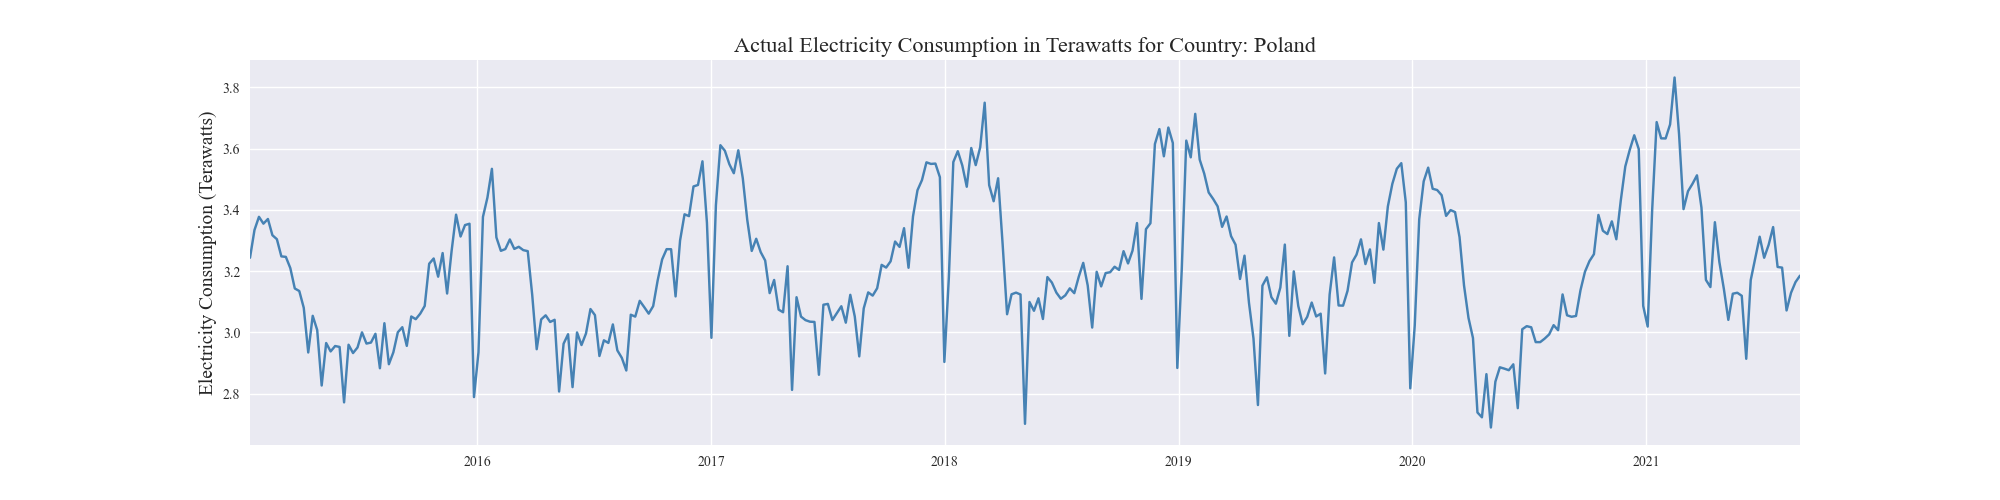
\includegraphics[width=\textwidth]{./out_figures/actual_electricity_consumption_Poland.png}
  \end{subfigure}

  \captionsetup{margin=10pt,font=small,labelfont=bf,width=.8\textwidth}

  \caption[Zużycie energii elektrycznej w Polsce, w okresie od 2015-01-01 do 2021-08-30. Dane zagregowane do tygodnia.]{Zużycie energii elektrycznej w Polsce, w okresie od 2015-01-01 do 2021-08-30. Dane zagregowane do tygodnia. \textit{Źródło:} opracowanie własne}\label{fig:x11}
\end{figure}



\subsection{Braki danych}

Na 2~161~177 rekordów, odnotowano 41~902 wierszy z brakującymi danymi dotyczącymi faktycznego zużycia prądu, co stanowi 1,94\% danych. W tabeli~\ref{tab:tabela4} przedstawiono procentowy udział braków danych dla każdego z krajów. 

\begin{table}[hbt]
  \centering

  \captionsetup{margin=10pt,font=small,labelfont=bf,width=.8\textwidth}

  \caption[Procentowy udział braków danych w badanych krajach EU.]{Procentowy udział braków danych w badanych krajach EU. \textit{Źródło:} opracowanie własne.}
  \label{tab:tabela4}
  
  \footnotesize

\vspace*{2ex}

\input{.//out\_tables//tab\_04.tex}

\end{table}

Analizując dane zamieszczone w tabeli~\ref{tab:tabela4} można zauważyć, że w większości państw procent pustych wartości jest nieznaczny i mieści się w przedziale od 0,00\% do 1,69\%. Wyróżniającym się krajem jest Cypr, gdzie odsetek brakujących danych wynosi aż 30,53\%.

W trakcie dalszej analizy brakujących danych skupiono się na lepszym zrozumieniu ich rozkładu. Przeprowadzono analizę częstotliwości występowania okresów czasu bez danych oraz ich długości, przy zagregowaniu danych do pełnych dni. Badanie miało na celu ustalenie, czy braki te to pojedyncze przypadki, czy też skupione są w dłuższych, ciągłych okresach. W tabeli~\ref{tab:tabela5} na stronie \pageref{tab:tabela5} w dodatku~\ref{sec:dodatek1}, przedstawiono wyniki tej analizy. 

Na podstawie analizy informacji dostępnych w tabeli~\ref{tab:tabela5} zauważono, że dla Cypru istnieje znaczący okres braków danych od 1 stycznia 2015 r. do 21 września 2016 r., obejmujący znaczną liczbę 630 dni. Ponadto, zidentyfikowano kilka krótszych przerw, takich jak okres od 8 czerwca 2019 r. do 23 lipca 2019 r. trwający 46 dni, oraz od 13 marca 2020 r. do 5 kwietnia 2020 r. trwający 24 dni. W związku z tym należy rozważyć, czy identyfikowane okresy występowania braków danych mogą mieć wpływ na jakość wyników modeli predykcyjnych dla Cypru.

W przypadku Luksemburga zidentyfikowano dwie przerwy w odnotowywaniu pomiarów. Pierwsza trwała 2 dni, miała miejsce 3--4 stycznia 2019 r., natomiast druga trwała 7 dni, od 31 stycznia 2019 r. do 6 lutego 2019 r. Również dla Rumunii rozpoznano trzy okresy braków danych: 1--5 stycznia 2015 r. trwający 5 dni, 22--23 maja 2018 r. trwający 2 dni oraz 7--9 sierpnia 2021 r. trwający 3 dni. W innych analizowanych krajach występowały krótsze przerwy, trwające od 2 do 8 dni. Poznanie tych okresów jest kluczowe dla zrozumienia kontekstu danych oraz potencjalnych działań, które mogą być podjęte w celu uzupełnienia brakujących informacji.

\subsection{Imputacja braków w danych}

W analizie szeregów czasowych wykluczenie niekompletnych obserwacji może spowodować uszkodzenie struktur czasowych, takich jak autokorelacja, trendy i sezonowość \citep{box1994}, dlatego istotna jest właściwie przeprowadzona imputacja brakujących danych uwzględniająca wspomniane cechy czasowe. 

W ramach tego badania postanowiono zastosować uzupełnianie brakujących danych poprzez średnią z 30 poprzednich pomiarów dla analogicznego dnia tygodnia i godziny. Taka metoda umożliwia uwzględnienie zarówno zmian związanych z porą dnia i dniem tygodnia, jak również sezonowymi trendami występującymi w różnych okresach roku. Na wykresie~\ref{fig:x12} przedstawiono szereg czasowy uwzględniający uzupełnione braki danych dotyczącego zużycia energii elektrycznej w Irlandii.

\begin{figure}[hbt]
  \centering

  \begin{subfigure}[t]{0.95\textwidth}
    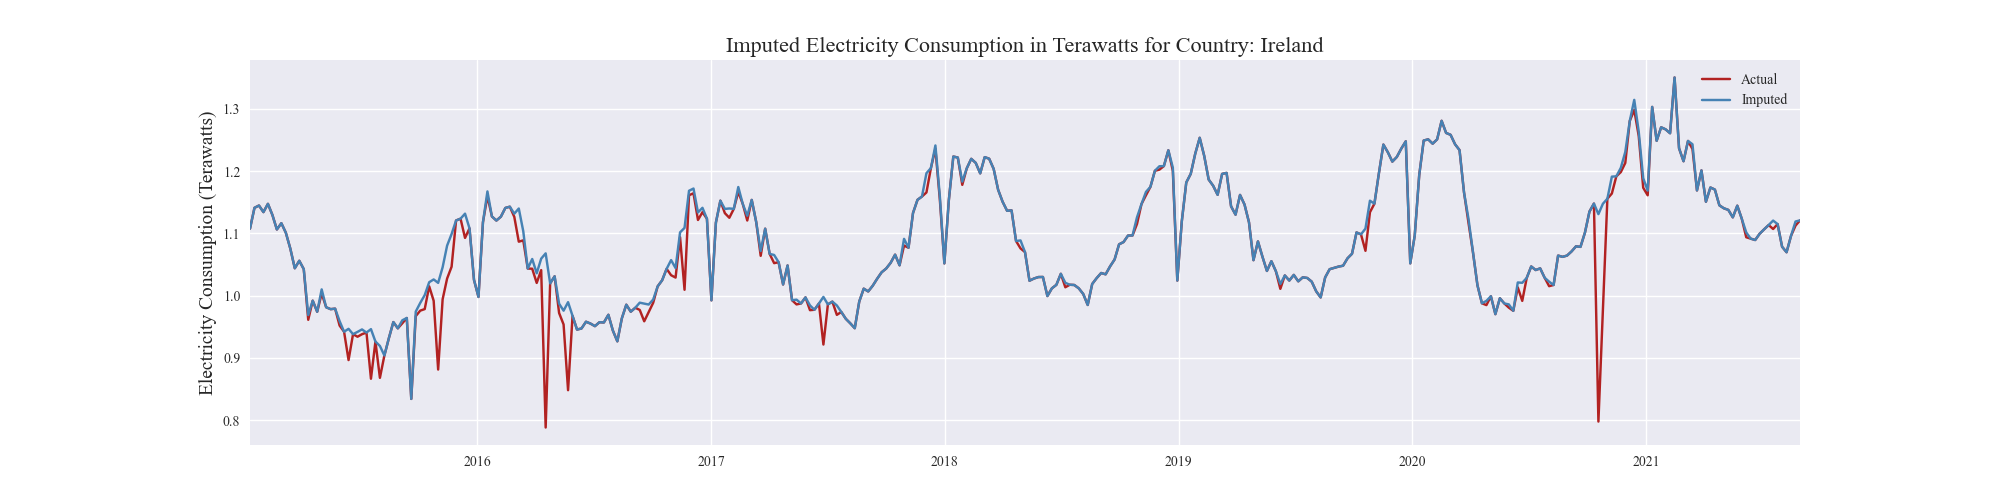
\includegraphics[width=\textwidth]{./out_figures/imputed_electricity_consumption_Ireland.png}
  \end{subfigure}

  \captionsetup{margin=10pt,font=small,labelfont=bf,width=.8\textwidth}

  \caption[Imputacja brakujących danych dotyczących zużycia energii elektrycznej w Irlandii, w okresie od 2015-01-01 do 2021-08-30. Dane zagregowane do tygodnia.]{Imputacja brakujących danych dotyczących zużycia energii elektrycznej w Irlandii, w okresie od 2015-01-01 do 2021-08-30. Dane zagregowane do tygodnia. \textit{Źródło:} opracowanie własne}\label{fig:x12}
\end{figure}

Proces imputacji brakujących danych został przeprowadzony oddzielnie dla każdego z badanych krajów UE, na niezagregowanych danych po procesie wstępnego przygotowania opisanym w podrozdziale~\ref{przygotowanie-danych}. W wyniku procesu imputacji brakujących danych ze zmiennej \code{TotalLoad_Actual_MW} utworzono nową zmienną o nazwie \code{TotalLoad_Imputed_MW} uzupełnioną o brakujące wartości. W ostatnim kroku przygotowania danych do wykorzystania podczas trenowania i testowania modeli predykcyjnych usunięto zmienną \code{TotalLoad_Actual_MW}, pozostawiając zmienne: \code{Country}, \code{Date} oraz \code{TotalLoad_Imputed_MW}. Przykładowe dane po zakończeniu imputacji braków danych zostały przedstawione w tabeli~\ref{tab:tabela5}.

\begin{table}[hbt]
  \centering

  \captionsetup{margin=10pt,font=small,labelfont=bf,width=.8\textwidth}

  \caption[Przykładowe wartości danych przygotowanych do zastosowania w modelowaniu prognostycznym.]{Przykładowe wartości danych przygotowanych do zastosowania w modelowaniu prognostycznym.. \textit{Źródło:} opracowanie własne.}
  \label{tab:tabela5}
  
  \footnotesize

\vspace*{2ex}

\input{.//out\_tables//tab\_07.tex}

\end{table}

\subsection{Ostateczne przygotowanie danych}

W niniejszym badaniu do trenowania i testowania modeli predykcyjnych wykorzystano dane zagregowane do tygodnia. Do agregacji danych wykorzystano wbudowaną w Python metodę \code{groupby}, która w połączeniu z metodą \code{sum} grupuje dane w ramce danych według zmiennej \code{Country}. Następnie wybrana zmienna, \code{TotalLoad_Imputed_MW}, jest sumowana dla każdej grupy. Dodatkowo, użyto metody \code{resample('W')} w celu zmiany częstotliwości próbkowania danych na tygodniową. W bibliotece \code{pandas} tydzień domyślnie zaczyna się od poniedziałku, dlatego dane są agregowane od poniedziałku do niedzieli danego tygodnia, a daty przedstawione w wynikowej ramce danych zawsze odpowiadają niedzieli. Warto zauważyć, że metoda \code{resample('W')} w przypadku, gdy tydzień znajduje się na przełomie lat, przypisuje go do roku, w którym przypada większość dni z tego tygodnia. Po zakończeniu procesu agregacji usunięto pierwszą i ostatnią wartość dla każdego badanego kraju ze względu na sztucznie powstałe spadki. Pierwsza data w zbiorze to 2015-01-01, czyli czwartek, natomiast ostatnia to 2021-08-30, odpowiada poniedziałkowi. Oznacza to, że zarówno na początku jak i na końcu zbioru danych brakuje pełnych 7 dni z wartościami \code{TotalLoad\_Imputed\_MW}. W związku z tym metody wykorzystane do agregacji zsumowały jedynie dostępne wartości, co zaskutkowło zaniżeniem wyników dla tych tygodni. W ten sposób uzyskano agregację obciążeń energetycznych dla różnych krajów na tygodniowej podstawie (zob.~tabela~\ref{tab:tabela7}). 

\begin{table}[hbt]
  \centering

  \captionsetup{margin=10pt,font=small,labelfont=bf,width=.8\textwidth}

  \caption[Przykładowe obserwacje z pliku \code{entsoe\_country.csv} po przygotowaniu i agregacji danych.]{Przykładowe obserwacje z pliku \code{entsoe\_country.csv} po przygotowaniu i agregacji danych. \textit{Źródło:} opracowanie własne.}
  \label{tab:tabela7}
  
  \footnotesize

\vspace*{2ex}

\input{.//out\_tables//tab\_07.tex}

\end{table}

Zbiór danych treningowych, odpowiadający w niniejszym badaniu okresowi przed pandemią COVID-19, obejmował zakres dat od 2015-01-11 do 2019-12-29. Wyjątkiem jest tutaj Cypr, dla którego zbiór treningowy zaczynał się od 2016-09-21 ze względu na znaczną ilość brakujących danych. 

% --- chapter ---------------------------------------------------------
\clearpage
\section{Wykorzystane metody}\label{sec:metody}

Do przeprowadzenia niniejszego badania wybrano trzy modele predykcyjne mające zastosowanie w prognozowaniu szeregów czasowych: SARIMA, TBATS oraz LSTM. Ze względu na małą ilość danych (347 cotygodniowych pomiarów dla każdego kraju), zdecydowano się pominąć etap walidacji. Każdy z tych modeli, dla każdego z badanych państw, został wytrenowany i przetestowany na danych przygotowanych do tych procesów (szczegółowe etapy przygotowania danych zostały omówione w rozdziale~\textit{\nameref{sec:dane}}). W celu pełnego zrozumienia efektywności każdego z wytrenowanych modeli, dokonano obliczeń metryk, takich jak MAPE, ME, MAE, MSE i RMSE. Wyniki tych obliczeń zostały udostępnione w załączniku, chociaż praca nie koncentruje się na bezpośrednim porównaniu skuteczności poszczególnych modeli.

\subsection{SARIMA}

W prognozowaniu szeregów czasowych modele ARIMA są jednymi z najczęściej używanych modeli, które dają obiecujące rezultaty \citep{elsaraiti2021}. Modele należące do tej grupy wykorzystują proces autoregresji \code{AR} (ang. \textit{autoregressive}), proces średniej ruchomej \code{MA} (ang. \textit{moving average}) oraz proces integracji \code{I} (ang. \textit{integrated}), dzięki czemu dobrze sobie radzą z prognozowaniem szeregów czasowych. Model SARIMA (Seasonal AutoRegressive Integrated Moving Average) jest rozszerzeniem modelu ARIMA o uwzględnienie sezonowości, co dodatkowo zwiększa jego skuteczność w modelowaniu szeregów czasowych, które wykazują regularne wzorce sezonowe~\citep{montgomery2011}. 

Wszystkie etapy badania dotyczące modelu SARIMA, poza analizą porównawczą między modelami, zawarto w autorskiej funkcji \code{sarima\_split\_best\_params\_search\_fit\_predict\_plot}. Jako argumenty wejściowe przyjmuje ona nazwę kraju oraz szereg czasowy dla tego kraju. Funkcja ta uruchamiana jest w pętli, dla każdego badanego kraju. W pierwszym kroku funkcja iteruje przez różne kombinacje parametrów modelu SARIMA: \code{p}, \code{d}, \code{q}, \code{P}, \code{D}, \code{Q} przy założone rocznej sezonowości. Optymalne parametry są wybierane na podstawie kryterium informacyjnego Akaike (AIC). Parametry nie różnią się między krajami i wynoszą \code{p = 0}, \code{d = 1}, \code{q = 0}, \code{P = 1}, \code{D = 1}, \code{Q = 1} i \code{s = 52}, który odpowiada liczbie okresów w sezonie (w tym przypadku --- liczbie tygodni w roku), co oznacza sezonowość roczną. Następnie korzystając z uzyskanych w poprzednim kroków parametrów, model SARIMA zostaje poddany procesowi treningu na danych z okresu sprzed pandemii (do końca roku 2019) i zapisany w formacie \code{.pkl}, po czym następuje etap predykcji. Kolejną częścią funkcji jest wygenerowanie i zapisanie wykresów porównujących dane rzeczywiste z prognozowanymi w formacie \code{.png}. W ostatnim etapie obliczane są metryki MAPE, ME, MAE, MSE i RMSE, które są zwracane przez funkcję w formie słownika \code{results}, wraz z prognozowanymi wartościami \code{yhat} i optymalnymi parametrami dla tego kraju \code{best_params}.
	
\subsection{TBATS}

TBATS (Trigonometric Exponential smoothing state space model with Box-Cox transformation, ARMA errors, Trend and Seasonal components) to model, który został zaprojektowany do prognozowania szeregów czasowych z wieloma okresami sezonowymi. Stosuje się w nim transformację Boxa-Coxa do oryginalnego szeregu czasowego, a następnie modeluje go jako liniową kombinację wygładzonego wykładniczo trendu, składowej sezonowej i składowej ARMA \citep{delivera2010}. Składowe sezonowe są modelowane za pomocą funkcji trygonometrycznych za pośrednictwem szeregów Fouriera. Dodatkowo TBATS przeprowadza pewne dostosowania hiperparametrów (np. które z tych składników zachować, a które odrzucić) przy użyciu kryterium informacyjnego Akaikego --- AIC \citep{hyndman2014}. Model ten  wykazuje skuteczność w uwzględnianiu wielu sezonowości obecnych w danych o charakterze dziennym i tygodniowym, o czym pisze w swojej publikacji \cite{montero2020}.

W podobny sposób jak w przypadku modelu SARIMA, analizę modelu TBATS przeprowadzono przy użyciu dedykowanej funkcji \code{tbats_split_best_params_search_fit_predict_plot}. W ramach tej funkcji, która przyjmuje nazwę kraju oraz szereg czasowy jako argumenty wejściowe, iteracyjnie przeprowadzano proces szukania optymalnych parametrów. Na tym etapie funkcja sprawdza różne kombinacje parametrów modelu TBATS, takie jak \code{seasonal_periods}, \code{use_arma_errors}, \code{use_box_cox_options}, \code{use_trend_options}, \code{n_jobs_option}, \code{use_damped_trend}, a ostateczny zestaw parametrów zostaje wybrany na podstawie minimalizacji kryterium informacyjnego Akaike (AIC). Jak widać w tabeli~\ref{tab:tabela9} parametr \code{use_arma_errors} nie różni się między krajami i jest równy \code{true}. W modelu użyto również dwóch stałych parametrów: \code{s = 52}, który odpowiada liczbie okresów w sezonie, w tym przypadku reprezentującej liczbę tygodni w roku i \code{n_jobs_option = 4}.

\begin{table}[hbt]
  \centering

  \captionsetup{margin=10pt,font=small,labelfont=bf,width=.8\textwidth}

  \caption[Najlepsze parametry do modelu TBATS, wybrane za pomocą funkcji \code{tbats\_split\_best\_params\_search\_fit\_predict\_plot}.]{Najlepsze parametry do modelu TBATS, wybrane za pomocą funkcji  \code{tbats\_split\_best\_params\_search\_fit\_predict\_plot}. \textit{Źródło:} opracowanie własne.}
  \label{tab:tabela9}
  
  \footnotesize

\vspace*{2ex}

\input{.//out\_tables//tab\_09.tex}

\end{table}

Analizując tabelę~\ref{tab:tabela9} można zwrócić uwagę na parametry niestałe takie jak \code{use_box_cox_options} i \code{use_trend_options}, które różnią się w zależności od badanego kraju. Parametr \code{use_box_cox_options} decyduje o tym, czy model będzie stosował transformację Boxa-Coxa na szereg czasowy. Szczególnie korzystne jest to w przypadku niestabilnej wariancji danych, gdzie transformacja może poprawić jakość modelu. Z kolei, parametr \code{use_trend_options} decyduje, czy model uwzględnia długoterminowe zmiany poprzez aktywację składnika trendu. Umożliwia to analizę ogólnych kierunków ewolucji danych na przestrzeni czasu, wpływając na dokładność prognoz. W dalszych krokach funkcja \code{tbats_split_best_params_search_fit_predict_plot} dzieliła dane na okres przed pandemią (zbiór treningowy) i po pandemii (zbiór testowy), trenowała model TBATS na danych sprzed pandemii, dokonywała prognoz, generowała wykresy porównawcze oraz obliczała metryki, takie jak MAPE, ME, MAE, MSE i RMSE. Ostatecznie funkcja zwraca wyniki \code{results}, prognozy (\code{yhat}), oraz optymalne parametry dla danego kraju (\code{best_params}).

\subsection{LSTM}

LSTM (Long Short-Term Memory) jest to rodzaj rekurencyjnej sieci neuronowej (RNN), będący zaawansowaną architekturą umożliwiającą skuteczne modelowanie długotrwałych zależności w danych sekwencyjnych. Wykorzystuje mechanizm bramek, takich jak bramki: wejściowa, wyjściowa i zapominająca, aby kontrolować przepływ informacji przez sieć, umożliwiając efektywne przechowywanie i wykorzystywanie informacji na różnych etapach sekwencji. Dzięki zdolnościom do skutecznego radzenia sobie z problemem zanikającego lub eksplodującego gradientu, sieć LSTM jest często stosowana w zadaniach prognozowania szeregów czasowych, przetwarzania języka naturalnego i innych obszarach, gdzie kluczowe są długoterminowe zależności \citep{geron2020}.  Decyzję o wykorzystaniu modelu LSTM jako kluczowego elementu w tej pracy badawczej podjęto na podstawie pracy \citep{siami-namini2018}, gdzie pokazano znaczącą skuteczność sieci LSTM w porównaniu do tradycyjnych algorytmów.

Sieci neuronowe, zwłaszcza modele rekurencyjne takie jak LSTM, wymagają zmiany formatu danych na sekwencje, aby efektywnie wykorzystać ich strukturę rekurencyjną i uwzględnić zależności czasowe między wartościami. W związku z tym, przed przystąpieniem do trenowania i testowania modelu LSTM konieczny był etap dodatkowego przygotowania danych. Zastosowano autorską funkcję \code{prepare_data} przyjmującą dwa argumenty wejściowe: \code{data} z szeregiem czasowym, oraz \code{look_back} z domyślną wartością równą 10. Ze względu na wartość \code{look_back}, która odpowiada 10 tygodniom niedostępnych danych (nie ma możliwości utworzenia pełnego 10-tygodniowego okna czasowego), podjęto decyzję o przesunięciu granicy czasowej dzielącej dane na okres przed i po pandemii stosowaną w modelach SARIMA i TBATS z 2020-01-01 na 2019-10-22. Dzięki temu możliwe będzie porównanie wyników predykcji dla wszystkich trzech modeli od początku roku 2020. Poniżej przedstawiono kolejne etapy przetwarzania danych omawianych w ramach funkcji \code{prepare_data}.
\begin{enumerate}[label=\arabic*.,noitemsep]
	\item Funkcja używa pętli \code{for}, aby iterować przez całość szeregu czasowego z uwzględnieniem długości okna \code{look_back}. Iteracje obejmują zakres, w którym dla każdego kroku czasowego pobierane są dane wejściowe \code{X} i odpowiadające im wartości docelowe \code{y}.
	\item Dla każdego \code{i} w zakresie, \code{X.append(data[i:i + look_back])} pobiera sekwencję \code{look_back} kroków czasowych jako dane wejściowe. Oznacza to, że dla każdego punktu w czasie, tworzona jest sekwencja o długości \code{look_back} obejmująca poprzednie kroki czasowe.
	\item Wartość docelowa dla danej sekwencji, to wartość następnego kroku czasowego po sekwencji, pobierana za pomocą \code{y.append(data[i + look_back])}.
	\item Pobrane sekwencje \code{X} i odpowiadające im wartości \code{y} są konwertowane na tablice \code{numpy} za pomocą \code{np.array(X), np.array(y)}.
	\item Ostatecznie zwracane są dwie tablice: \code{X}, która zawiera sekwencje danych wejściowych, oraz \code{y}, która zawiera odpowiadające im wartości docelowe.
\end{enumerate}

Topologia wykorzystanej w tym badaniu sieci neuronowej obejmuje dwie warstwy LSTM z warstwami Dropout po obu z nich oraz jedną warstwę gęstą (Dense), tak jak przedstawiono w poniższym kodzie.
\begin{lstlisting}[language=Python, numbers=none]
model = Sequential()
model.add(LSTM(128, input_shape=(look_back, 1), return_sequences=True))
model.add(Dropout(0.2))
model.add(LSTM(64))
model.add(Dropout(0.2))
model.add(Dense(1))
model.compile(
    loss='mean_squared_error', 
    metrics=["mape", lstm_me], 
    optimizer='adam'
)
\end{lstlisting}	
Pierwsza warstwa LSTM zawiera 128 neuronów, co oznacza, że będzie miała 128 neuronów, które mogą przechowywać informacje o dłuższych zależnościach czasowych w danych. Przyjmuje wejście o wymiarach \code{(look_back, 1)}, co oznacza, że dane wejściowe są dwuwymiarowe, gdzie jeden wymiar reprezentuje ilość kroków czasowych \code{look_back = 10}, a drugi wymiar reprezentuje liczbę cech dla każdego kroku czasowego --- 1. Parametr \code{return_sequences=True} oznacza, że ta warstwa LSTM zwraca pełne sekwencje zamiast jedynie ostatniego stanu. W związku z tym, dla każdego punktu czasowego w sekwencji, warstwa ta zwraca wektor stanów o długości 128, czyli dwuwymiarową macierz o wymiarach (10, 128). 

Kolejną warstwą jest warstwa Dropout, która pomaga w regularyzacji modelu, eliminując losowo 20\% połączeń między neuronami, co pomaga zapobiegać przeuczeniu. Przyjmuje ona wyjście poprzedzającej ją warstwy (sekwencję stanów LSTM o kształcie \code{(10, 128)}), a jej wyjście będzie takie samo jak wejście, lecz z losowo usuniętymi połączeniami pomiędzy neuronami (w tym przypadku 20\% neuronów zostanie pominiętych). 

Trzecią warstwą jest kolejna warstwa LSTM, z 64 neuronami. Ta warstwa przyjmuje wynik warstwy poprzedzającej, o rozmiarze \code{10, 128)}. W tym przypadku nie użyto \code{return_sequences}, co oznacza, że ta warstwa LSTM nie zwraca całej sekwencji, ale tylko jej ostatni stan. Dlatego jej wyjście ma kształt jednowymiarowej sekwencji o długości 64 \code{(64,)}, gdzie każdy element reprezentuje stan po przetworzeniu danych przez 64 neurony tej warstwy. 

Następna warstwa to ponownie warstwa Dropout, wspomagająca regularyzację modelu. Tak jak w przypadku poprzedniej warstwy Dropout, eliminowane jest 20\% połączeń między neuronami. Tym razem przyjmuje ona jednowymiarową sekwencję o długości 64 \code{(64,)} będącą wyjściem poprzedniej warstwy, zwraca macierz o tym samym rozmiarze nie biorąc pod uwagę 20\% jednostek.

Ostatnia warstwa modelu --- warstwa gęsta (Dense) z jedną jednostką służy jako warstwa wyjściowa, generując prognozy. Przyjmuje ona wyjście z warstwy Dropout o rozmiarze \code{(64,)}. Wewnątrz tej warstwy następuje proces optymalizacji za pomocą algorytmu optymalizacji \code{adam}, który używa gradientów, aby zaktualizować wagi i biasy w kierunku minimalizacji funkcji straty (Mean Squared Error). Ostateczne wyjście z warstwy Dense to wynik zastosowania funkcji aktywacji na sumie iloczynu skalarnego wektorów wejścia i wag z wartością bias. W tym przypadku, ponieważ nie jest określona inna funkcja aktywacji, wyjście jest identyczne z wynikiem tego działania.

Sieć jest kompilowana z użyciem funkcji straty \code{mean_squared_error}, metryki \code{mape} (mean absolute percentage error) oraz optymalizatora \code{adam}. Średni błąd kwadratowy (MSE) jest często używany jako funkcja straty w sieciach neuronowych ze względu na kilka powodów. Po pierwsze, taka funkcja straty jest łatwa do zrozumienia i zaimplementowania, co wynika z jej silnych podstaw matematycznych, ułatwiających analizę teoretyczną i obliczeniową. Po drugie, minimalizowanie MSE prowadzi do zbieżności modelu do danych treningowych, a optymalizacja modelu w tym kierunku zmniejsza różnicę między prognozowanymi a rzeczywistymi wartościami. Po trzecie, MSE jest bardziej wrażliwe na większe błędy w prognozach, co może być korzystne w określonych sytuacjach. Ze względu na opisane powyżej cechy średniego błędu kwadratowego, podjęto decyzję o jego zastosowaniu jako funkcję straty w omawianej sieci LSTM. Średni procentowy błąd bezwzględny (MAPE) został wykorzystany jako narzędzie oceny skuteczności sieci LSTM z uwagi na jej kluczową rolę jako głównego kryterium porównawczego efektywności z pozostałymi modelami.

Optymalizator \code{adam} reprezentuje adaptacyjny algorytm optymalizacji stosowany głównie do szkolenia głębokich sieci neuronowych. Opiera się na kombinacji zalet dwóch popularnych metod optymalizacyjnych, AdaGrad i RMSProp, w celu efektywnej aktualizacji wag sieci. Kluczową cechą tego optymalizatora jest adaptacyjne dostosowywanie współczynnika uczenia się dla każdego parametru na podstawie pierwszego i drugiego momentu gradientu, co umożliwia bardziej elastyczne dostosowanie i przyspiesza proces konwergencji \citep{frackiewicz2023}.


% --- chapter ---------------------------------------------------------
\clearpage
\section{Uzyskane wyniki i dyskusja}\label{sec:wyniki}

W tym rozdziale przedstawione zostaną główne wyniki analizy, które miały na celu zbadanie wpływu wyboru modelu prognostycznego na oszacowanie skutków pandemii COVID-19 w kontekście zużycia energii elektrycznej. Badanie obejmowało prognozy dla 23 krajów UE, uwzględniając modele SARIMA, TBATS oraz LSTM. Przedstawione wyniki mają na celu odpowiedzieć na pytanie, jak różnice w modelach wpływają na oszacowanie zmian w zużyciu energii elektrycznej, ze szczególnym uwzględnieniem okresu pandemii w porównaniu do danych sprzed tego wydarzenia. 

\begin{figure}[hbt]
  \centering

  \begin{subfigure}[t]{0.95\textwidth}
    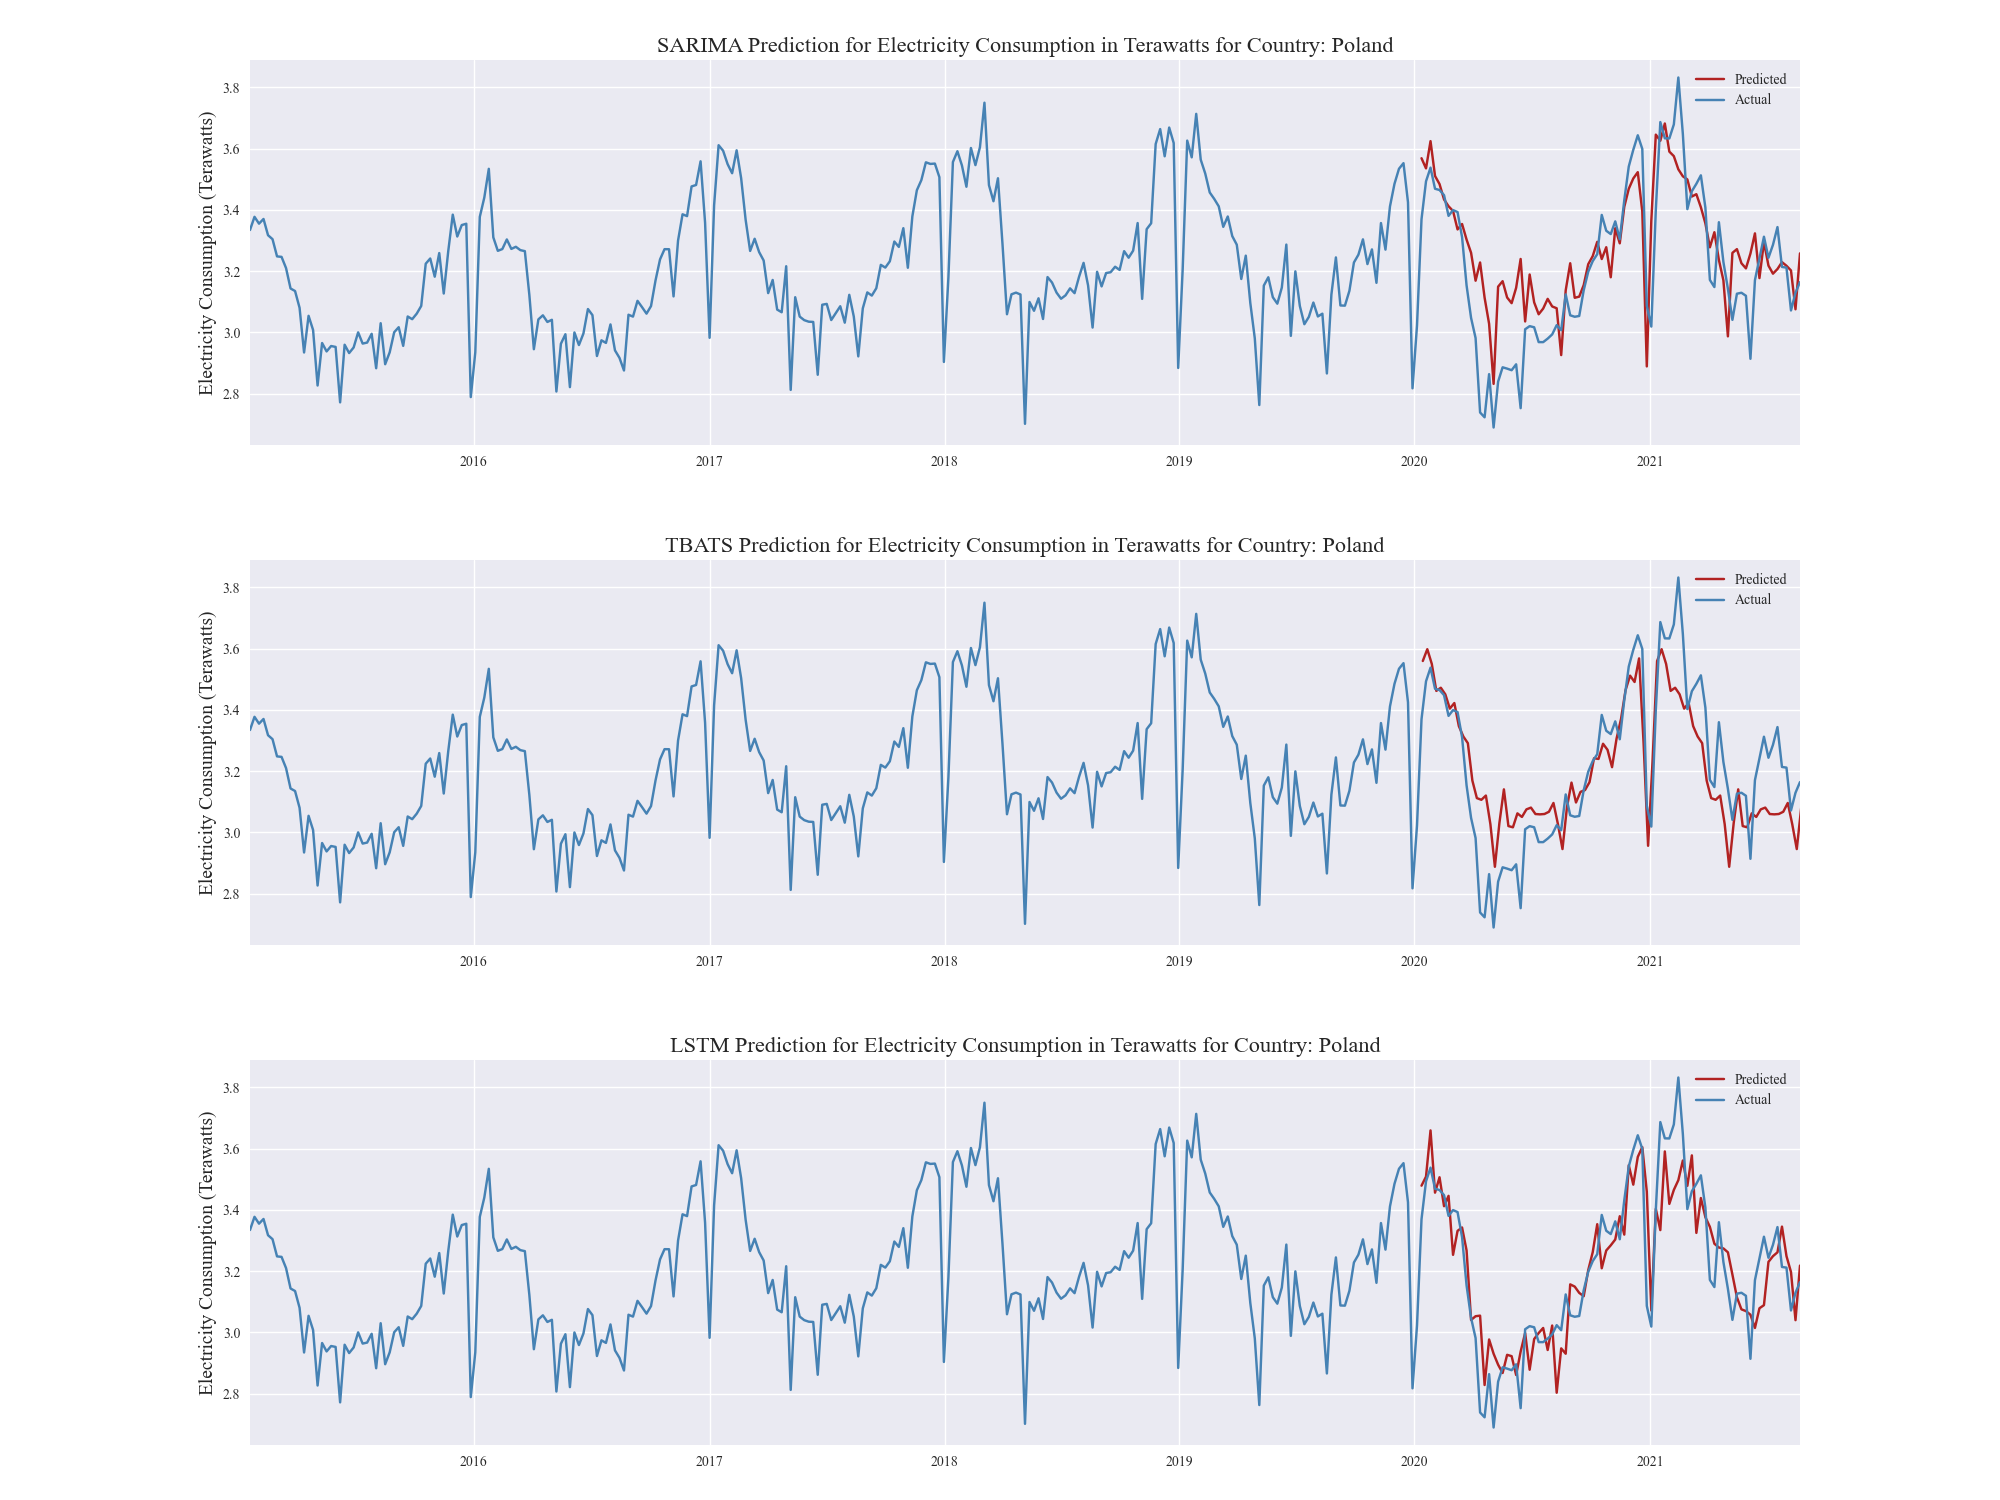
\includegraphics[width=\textwidth]{./out_figures/model_comparison_Poland.png}
  \end{subfigure}

  \captionsetup{margin=10pt,font=small,labelfont=bf,width=.8\textwidth}

  \caption[Porównanie predykcji trzech modeli (SARIMA, TBATS, LSTM) dla kraju Polska.]{Porównanie predykcji trzech modeli (SARIMA, TBATS, LSTM) dla kraju Polska. \textit{Źródło:} opracowanie własne}\label{fig:x13}
\end{figure}

Wykres~\ref{fig:x13} prezentuje wyniki predykcji na danych dotyczących zużycia energii elektrycznej w Polsce dla wszystkich trzech modeli wykorzystanych w badaniu. Analizując ten wykres można zauważyć, że model sieci neuronowej mało generalizuje predykcje, natomiast najlepiej wypada pod względem pokrywania się krzywej predykcji z krzywą odpowiadającą rzeczywistemu zapotrzebowaniu na prąd. Dane prognozowane przez model TBATS mają najmniej pików, co skłania do wniosku, że proces generalizacji w tym przypadku wypada najkorzystniej i jest mniejsza szansa na zjawisko \textit{overfitting'u}. W przypadku predykcji modelu SARIMA krzywa danych prognozowanych najmniej nakłada się na krzywą z danymi rzeczywistymi, odnotowano również nieregularne piki.

Kolejnym aspektem, na który warto zwrócić uwagę patrząc na wykres~\ref{fig:x13} jest gwałtowny, utrzymujący się spadek zużycia energii elektrycznej mający miejsce w drugim kwartale 2020 roku. Odpowiada on okresowi, w którym w Polsce został wprowadzony tzw. lockdown i pokazuje jak duży wpływ na zużycie prądu miał początkowy okres pandemii COVID-19. Dodatkowo, w pierwszym kwartale roku 2021 odnotowano duży skok zapotrzebowania na energię elektryczną. Podobne odczyty świadczące o, kolejno, obniżonej i zwiększonej konsumpcji energii elektrycznej w tych okresach odnotowano dla większości z badanych państw. 

Warto zauważyć, że z prognoz przedstawionych na wykresie~\ref{fig:x13} tylko sieć LSTM uwzględnia tak duży spadek zużycia energii elektrycznej. Biorąc pod uwagę fakt, że wszystkie modele były trenowane na danych nieobarczonych analogicznymi nagłymi sytuacjami kryzysowymi, można tą część prognozy uznać za błędnie zaniżoną --- model ten nie miał podstaw do oszacowania tak dużego spadku. Inaczej sytuacja wygląda dla skoku zużycia energii elektrycznej na początku 2021 roku --- w tym przypadku żaden z badanych modeli nie przewidział tego zwiększenia konsumpcji prądu.

W celu dokładniejszej analizy modelu LSTM wygenerowano wykres~\ref{fig:x14} przedstawiający funkcję straty (MSE), uwzględniając dane dla Polski. W przypadku sieci neuronowych jest to istotnym wyznacznik ich efektywności. Prawidłowo wyglądający wykres funkcji straty w kontekście uczenia maszynowego zazwyczaj przedstawia kilka charakterystycznych cech:

\begin{itemize}[noitemsep]
	\item gwałtowny spadek na początku --- na początku treningu modelu funkcja straty powinna gwałtownie maleć, co świadczy o tym, że model szybko uczy się dostosowywać do danych treningowych;
	\item stabilizacja --- po początkowym spadku, funkcja straty powinna się ustabilizować, co oznacza, że model osiągnął pewien stopień nauki i nie ma już dużych zmian w skuteczności;
	\item brak gwałtownych skoków --- w miarę upływu epok treningowych funkcja straty powinna utrzymywać się na stosunkowo stałym poziomie, a nie wykazywać gwałtownych skoków, co sugerowałoby problemy z modelem;
\end{itemize}
Opisane powyżej charakterystyki wynikają z procesu optymalizacyjnego sieci neuronowych, które starają się minimalizować wartości wybranej funkcji straty. Ma tu zastosowanie podejście prymitywne: w ostatniej warstwie sieci obliczany jest wynik funkcji straty, następuje zmiana wag neuronów i ponowne wyliczenie funkcji straty biorąc pod uwagę nowe wagi. W przypadku odnotowania spadku wartości funkcji straty sieć kontynuuje zmiany w obranym w poprzednim kroku kierunku \citep{brzezinski2021}. 

Patrząc na wykres~\ref{fig:x14} można zauważyć, że spełnia on wszystkie przedstawione wyżej kryteria, a co za tym idzie wykorzystaną w badaniu sieć neuronową w przypadku tego kraju można byłoby określić mianem efektywnej. W przypadku Polski wykres funkcji straty dla badanej sieci LSTM zaczęła się stabilizować po mniej-więcej 200 epokach.
\begin{figure}[hbt]
  \centering

  \begin{subfigure}[t]{0.95\textwidth}
    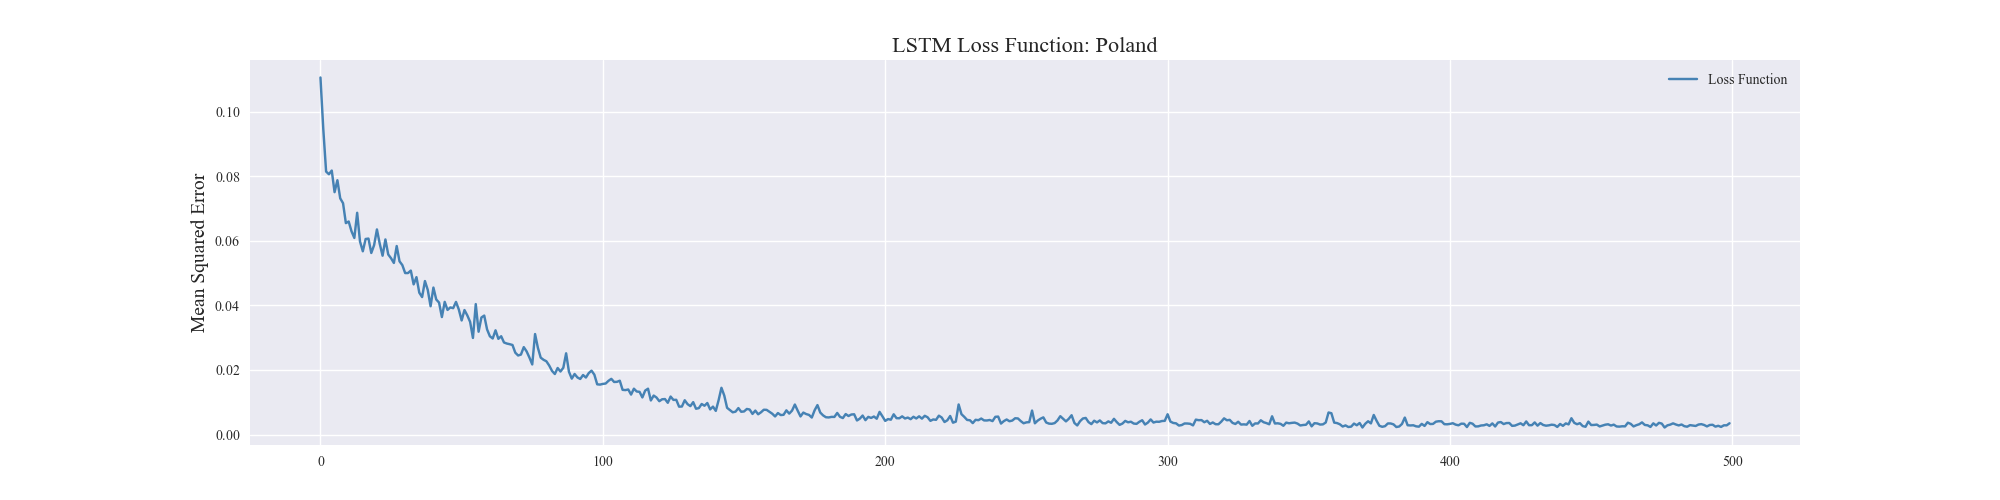
\includegraphics[width=\textwidth]{./out_figures/lstm_loss_function_Poland.png}
  \end{subfigure}

  \captionsetup{margin=10pt,font=small,labelfont=bf,width=.8\textwidth}

  \caption[Funkcja straty MSE dla modelu LSTM dla kraju Polska.]{Funkcja straty MSE dla modelu LSTM dla kraju Polska. \textit{Źródło:} opracowanie własne}\label{fig:x14}
\end{figure}

Założeniem pracy jest pokazanie jak bardzo różnią się oszacowania spadków zapotrzebowania na moc w czasie pandemii w zależności od wykorzystanego modelu prognostycznego. W tym celu przeprowadzono analizę porównawczą różnic między rzeczywistymi a prognozowanymi wartościami zużycia prądu w danym kraju wyrażonych w procentach, dla każdego z wykorzystanych modeli predykcyjnych. W tabeli~\ref{tab:tabela12} przedstawione zostały maksymalne odnotowane wartości bezwzględne błędów wyrażone w procentach dla poszczególnych modeli oraz dla każdego z analizowanych krajów. Najwyższe różnice odnotowano dla Cypru (SARIMA: 41,31\%, TBATS: 60,68\%, LSTM: 44,70\%), co potwierdza tezę mówiącą o zauważalnie gorszej jakości predykcji, kiedy występuje znaczny odsetek braków danych (w przypadku tego kraju wynosił on 30,53\%). Ze względu na odstające od reszty braki danych i wyniki zdecydowanie odbiegające od pozostałych, ten kraj został wyłączony z dalszych analiz. Najwyższe błędy w następnej kolejności odnotowano dla modelu SARIMA i odpowiadają one wartościom: 39,63\% (Włochy), 36.27\% (Estonia) i 34.70\% (Grecja). Maksymalnie odnotowane błędy procentowe dla tego modelu nie przekroczyły 15\% tylko dla Irlandii (13,85\%), podczas gdy w przypadku zarówno TBATS jak i LSTM odnotowano 9 krajów mieszczących się w tym zakresie. 

\begin{table}[hbt]
  \centering

  \captionsetup{margin=10pt,font=small,labelfont=bf,width=.8\textwidth}

  \caption[Maksymalne odnotowane błędy procentowe dla poszczególnych modeli i krajów.]{Maksymalne odnotowane błędy procentowe dla poszczególnych modeli i krajów. \textit{Źródło:} opracowanie własne.}
  \label{tab:tabela12}
  
  \footnotesize

\vspace*{2ex}

\input{.//out\_tables//tab\_12.tex}

\end{table}

Wykres~\ref{fig:x15} przedstawia porównawczą analizę błędów prognoz dla Polski wyrażoną w procentowej różnicy między danymi rzeczywistymi a prognozowanymi, uwzględniającą modele SARIMA, TBATS i LSTM w kontekście ich ewolucji w czasie. Zauważalny jest wzrost wartości błędów w dwóch omawianych już wcześniej okresach: drugi kwartał 2020 roku, oraz pierwszy kwartał 2021 roku. Wykres ten potwierdza uprzednie spostrzeżenia --- sieć LSTM ma najniższe wartości błędów, nie odnotowano też znacznego skoku w okresie związanym z lockdownem, co biorąc pod uwagę dane przed pandemiczne użyte do trenowania sugeruje, że nie zadziałała ona prawidłowo, zaniżając prognozy. Modelem który wyróżnia się pod względem wysokości błędów jest SARIMA, co potwierdza informacje zamieszczone w tabeli~\ref{tab:tabela12}. TBATS jako jedyny z badanych modeli zachował się przewidywalnie --- cechował się stosunkowo niskimi błędami prognoz, przy czym zareagował na oba niewystępujące w okresie przed pandemią wahania zgodnie z oczekiwaniami,  zwiększeniem wartości błędu.

\begin{figure}[hbt]
  \centering

  \begin{subfigure}[t]{0.95\textwidth}
    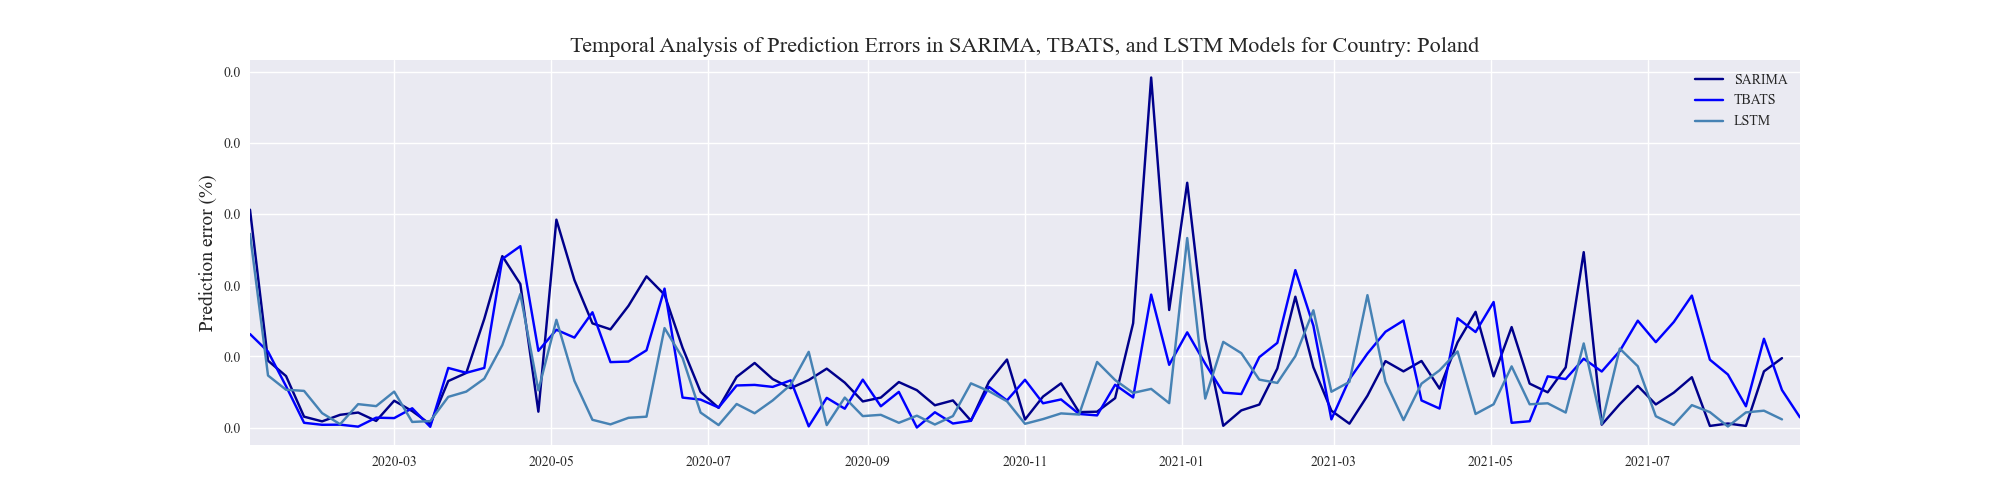
\includegraphics[width=\textwidth]{./out_figures/maximum_percentage_error.png}
  \end{subfigure}

  \captionsetup{margin=10pt,font=small,labelfont=bf,width=.8\textwidth}

  \caption[Rozwój w czasie błędów prognoz: Analiza porównawcza modeli SARIMA, TBATS i LSTM dla Polski.]{Rozwój w czasie błędów prognoz: Analiza porównawcza modeli SARIMA, TBATS i LSTM dla Polski. \textit{Źródło:} opracowanie własne}\label{fig:x15}
\end{figure}

Analizując powyższe wyniki nasuwa się wniosek, że żaden z badanych modeli nie poradził sobie z sytuacją związaną z wystąpieniem nagłego, nieprzewidzianego zdarzenia, w przypadku niniejszego badania --- wystąpienia pandemii COVID-19. Podobne obserwacje wysnuł \cite{abutalib2023} w swoim badaniu. Oceniał on wpływ COVID-19 na wydajność modeli sztucznej inteligencji analizując wpływ różnych czynników zewnętrznych na wzorce konsumpcji wody. Wykazał, że modele prognozowania osiągnęły wysoką dokładność przed pandemią, ale zanotowano spadek po jej rozpoczęciu, co daje przestrzeń do dalszych badań związanych z wydajnością modeli predykcyjnych w przypadku wystąpienia nieprzewidzianych zdarzeń. Istnieje wiele technik mających na celu zwiększenie skuteczności. Pierwszą z nich jest odpowiedni dobór modelu predykcyjnego --- \cite{abutalib2023} wykazał, że modele ensemble wykazywały największą adaptacyjność do nieregularnej konsumpcji w okresie pandemii COVID-19, dlatego warto rozważyć ich zastosowanie i dalszą optymalizację. Kolejnym ważnym aspektem jest zwiększenie i regularne aktualizowanie zbioru treningowego o aktualne dane zawierające takie nieprzewidziane zmiany. Istotny jest również dobór czynników, które są uwzględniane przez model podczas predykcji, co podkreśla \cite{jasiński2014} w swojej pracy badawczej:

\enquote{Podstawowym elementem wpływającym na jakość uzyskiwanych wyników jest zestaw zmiennych objaśniających. Badania empiryczne i te o charakterze literaturowym wykazały, że można odnaleźć wiele różnych kombinacji wejściowych szeregów czasowych, na podstawie których można dokonać poprawnych symulacji}.

Istnieje szereg elementów mających wpływ na prognozowane zapotrzebowanie na energię w przyszłości. Do kluczowych czynników zalicza się aspekty czasowe, takie jak godzina, dzień tygodnia, numer tygodnia, miesiąc czy rok, a także charakterystyka konkretnego dnia oraz wskaźniki sezonowe. Ponadto, istotne są zarówno przeszłe, jak i prognozowane rezerwy, historyczne ceny, poprzednie oraz przewidywane zapotrzebowanie na energię. Warto uwzględniać także wymianę energii między sąsiednimi obszarami, zwłaszcza w kontekście umów długoterminowych, a także parametry klimatyczne, takie jak zmiany temperatury czy temperatura punktu rosy. Dodatkowym elementem jest cena innych surowców energetycznych, takich jak ropa czy gaz, oraz paliw. Można również dokonać podziału na dane opisujące rynek, obejmujące historię obciążenia, rezerwy, zdolności wytwórcze generatorów, import, eksport oraz ograniczenia przesyłowe linii. Niestrategiczna niepewność, a zwłaszcza prognozowane zapotrzebowanie, rezerwy, czynniki pogodowe i ceny innych surowców paliw, stanowi istotny element analizy. Ponadto, istnieje grupa czynników losowych, obejmująca przerwy w dostawach prądu, stan linii przesyłowych czy wskaźniki przeciążenia. W analizie rynku warto również uwzględnić wskaźniki zachowań rynkowych, takie jak przeszłe ceny, elastyczność popytu czy strategie akcyjne, a także elementy czasowe, w tym okresy rozliczeniowe i wcześniej wspomniane czynniki czasowe \citep{nejad2011, aggarwal2009}.

Kolejnym ważnym elementem jest implementacja mechanizmów uczenia ze wzmocnieniem, pozwala modelowi na dynamiczne dostosowywanie się do nieznanych wcześniej sytuacji. To elastyczne podejście umożliwia modelowi adaptację do zmieniających się warunków, co jest kluczowe dla skutecznego radzenia sobie z nieprzewidzianymi scenariuszami. Z kolei zastosowanie reaktywnej logiki umożliwi modelowi szybką reakcję na nieprzewidziane sytuacje. Ta zdolność do natychmiastowego dostosowywania się może być kluczowa dla utrzymania skuteczności modelu w dynamicznym środowisku, takim jak sektor energetyczny. Ważnym krokiem w utrzymaniu skuteczności jest także przeprowadzanie regularnych audytów, które pozwala identyfikować potencjalne obszary problematyczne lub zmiany w danych mogące wpłynąć na skuteczność modelu. Skutecznym podejściem jest również utworzenie systemu monitorowania wydajności modelu, który bieżąco informuje o występowaniu ewentualnych anomalii, co pozwala na szybką reakcję na nieprzewidziane zdarzenia, minimalizując negatywne skutki. Ostatecznie, kluczowe jest także uwzględnienie zestawu danych do testowania nieprzewidzianych sytuacji. Włączenie specjalnych zestawów danych testowych, które symulują nieprzewidziane sytuacje, umożliwia ocenę i doskonalenie zdolności modelu do prognozowania w warunkach, które nie były wcześniej uwzględnione. 

% --- chapter ---------------------------------------------------------
\clearpage
\section{Zakończenie}\label{sec:zakonczenie}

Podsumowując przeprowadzone badanie, a także jego wyniki i część dyskusyjną, głównym celem niniejszej pracy było przeprowadzenie analizy wpływu wyboru modelu prognostycznego na dokładność oszacowania skutków pandemii COVID-19 w kontekście prognozowania zużycia energii elektrycznej w Polsce. Z przeprowadzonej analizy wynika, że z perspektywy tego celu, najlepiej i najbardziej przewidywalnie zachował się model TBATS, podczas gdy na nieprzewidziane zmiany z najniższą skutecznością zareagowała metoda SARIMA. Badanie wykazało, że modele użyte w analizie charakteryzowały się ograniczoną skutecznością w przewidywaniu niespodziewanych zdarzeń, z wyjątkiem modelu LSTM w przypadku drugiego kwartału 2020 roku. Warto jednak zauważyć, że w tej sytuacji powodzenie predykcji sieci LSTM wynikało z błędu prognozy, a nie zdolności do faktycznego przewidzenia zmiany w zużyciu prądu. 

Analizowane prognozowane zapotrzebowanie na energię w przyszłości podlega wpływowi wielu czynników, takich jak aspekty czasowe, rezerwy, ceny historyczne, wymiana energii między obszarami, parametry klimatyczne, cena innych surowców energetycznych i paliw. Dodatkowo, istotne są czynniki rynkowe, takie jak obciążenie, rezerwy, zdolności wytwórcze, import, eksport, oraz elementy losowe, takie jak przerwy w dostawach prądu i wskaźniki przeciążenia, podczas gdy wskaźniki zachowań rynkowych i elementy czasowe również odgrywają kluczową rolę w analizie.

Rozważając możliwości optymalizacji modeli, warto zauważyć, że istnieje wiele metod, takich jak stosowanie modeli ensemble, dostosowywanie modelu do elastycznych struktur, dynamiczne aktualizacje na podstawie nowych danych, integracja zewnętrznych czynników czy stosowanie hybrydowych modeli, które mogą poprawić ogólną odporność modelu na zmienne warunki. Niemniej jednak, mimo coraz bardziej zaawansowanych technik prognostycznych, wciąż brakuje algorytmów, które skutecznie przewidują nieprzewidziane zdarzenia, zwłaszcza te, które nie zostały uwzględnione na etapie tworzenia modelu. To wskazuje na wyzwanie, przed jakim stoi dziedzina ekonometrii, szczególnie w kontekście dynamicznych sytuacji, gdzie tradycyjne modele mogą nie być wystarczająco elastyczne. Wnioski te podkreślają potrzebę dalszych badań i doskonalenia technik prognostycznych w celu rozwinięcia zdolności modeli do radzenia sobie z rzeczywistymi, nieoczekiwanymi zmianami w danych wejściowych.

% --- chapter ---------------------------------------------------------
\appendix
\clearpage
\section{Dodatkowe tabele}\label{sec:dodatek1}

\begin{table}[H]
  \centering

  \captionsetup{margin=10pt,font=small,labelfont=bf,width=.8\textwidth}

  \caption[Dane z pliku \code{entsoe\_country\_dict.csv}.]{Dane z pliku \code{entsoe\_country\_dict.csv}. \textit{Źródło:} opracowanie własne.}
  \label{tab:tabela2}
  
  \footnotesize

\vspace*{2ex}

\input{.//out\_tables//tab\_02.tex}

\end{table}



% --- bibliography ----------------------------------------------------
\clearpage
\bibliographystyle{agsm}
\bibliography{refs}

% --- abstract --------------------------------------------------------
\clearpage
\addcontentsline{toc}{section}{Lista tablic}
\listoftables

% --- abstract --------------------------------------------------------
\clearpage
\addcontentsline{toc}{section}{Lista rysunków}
\listoffigures



% --- abstract --------------------------------------------------------
\clearpage
\addcontentsline{toc}{section}{Streszczenie}
\section*{Streszczenie}

Głównym celem niniejszej pracy jest analiza wpływu wyboru modelu prognostycznego na dokładność oszacowania skutków pandemii COVID-19. Badanie zostało przeprowadzone na danych Europejskiego Systemu Operatorów Przesyłowych Energii Elektrycznej (ENTSOE) obejmujących 23 kraje Unii Europejskiej. Dla każdego z tych krajów zastosowano trzy różne modele prognostyczne: SARIMA, TBATS oraz LSTM. Podstawą do analizy było użycie danych sprzed pandemii, sięgających początku 2015 roku, w celu prognozowania zużycia energii elektrycznej na okres od 2020 roku. Badanie obejmowało szeroki zakres aspektów, od technicznych detali zastosowanych modeli po analizę wyników prognoz. Badanie wykazuje, że model TBATS zachował się najlepiej, metoda SARIMA reagowała z najniższą skutecznością na nieprzewidziane zmiany podczas gdy model LSTM niezgodnie z procesem trenowania zaniżył wartości prognoz na czas pandemii, przypadkowo dokonując prawidłowej prognozy. Odkrycia sugerują, że mimo zaawansowanych technik prognozowania, istnieje wyzwanie w skutecznym przewidywaniu nieoczekiwanych zdarzeń, szczególnie w dynamicznych sytuacjach, podkreślając potrzebę dalszych badań i doskonalenia technik prognostycznych.


\end{document}

%%% Local Variables:
%%% mode: latex
%%% TeX-master: t
%%% End:
